%!TEX root = paper.tex
\begin{figure}[ht]      
\centering
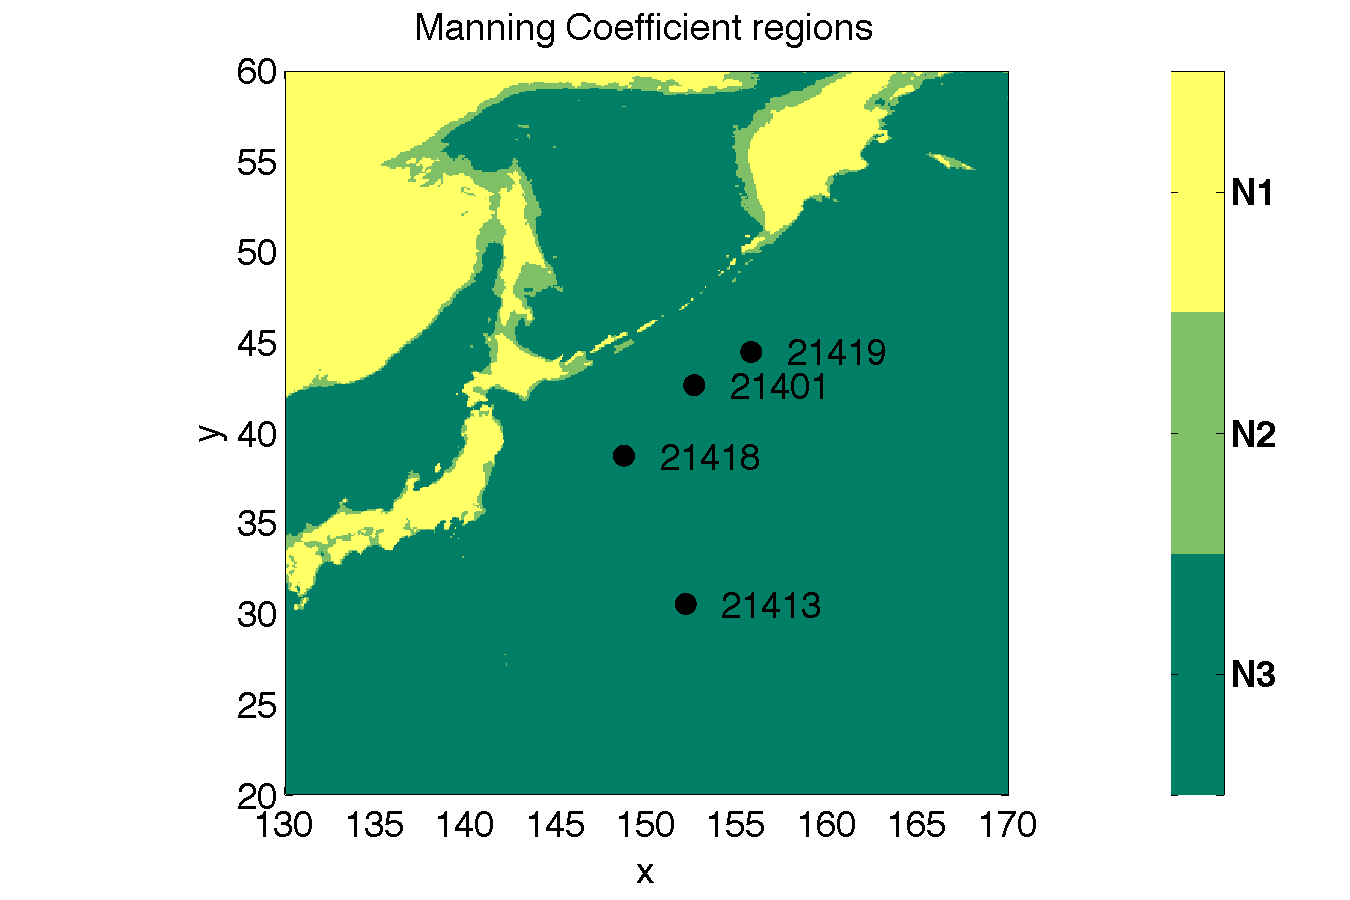
\includegraphics[width=0.6\textwidth]{./figures/coef.pdf}
\caption{Manning's $n$ coefficients at three regions: $n_1$ on-shore, $n_2$ near shore, $n_3$ deep-water.}
\label{fig:ceofs}
\end{figure}  
%%%%%%%%%%%%%%%%%%%%%%%%%%%%%%%%%%%%%%%%%%%%%%%%%%%%%%%%%%%%%%%%

\begin{figure}[ht]
\centering
\begin{subfigure}[c]{0.45\textwidth}
    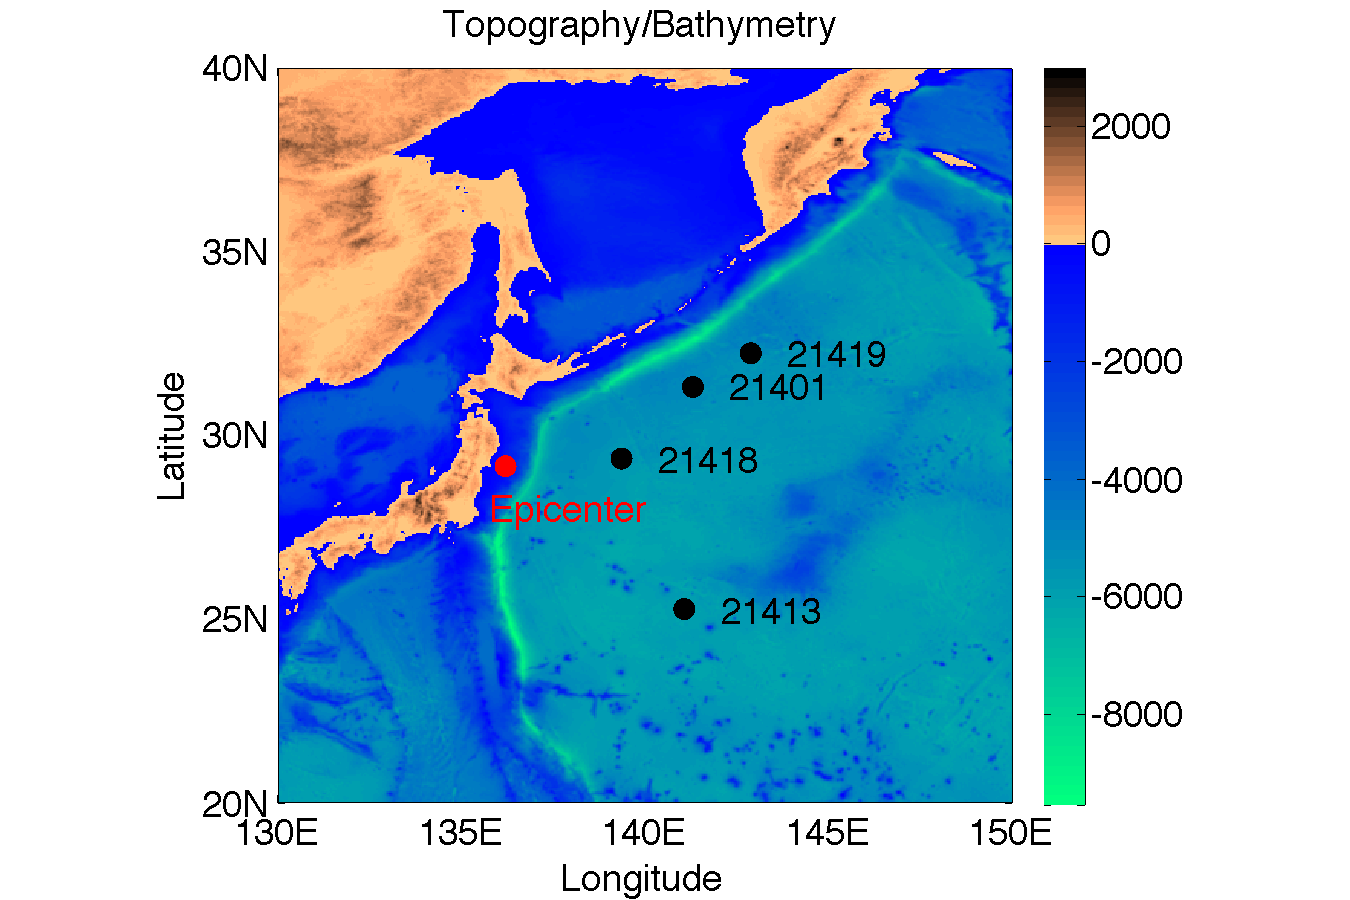
\includegraphics[width=\textwidth]{./figures/topo.pdf}
    \caption{} \label{fig:setup_buoy_locations}
\end{subfigure}
\begin{subfigure}[c]{0.45\textwidth}
    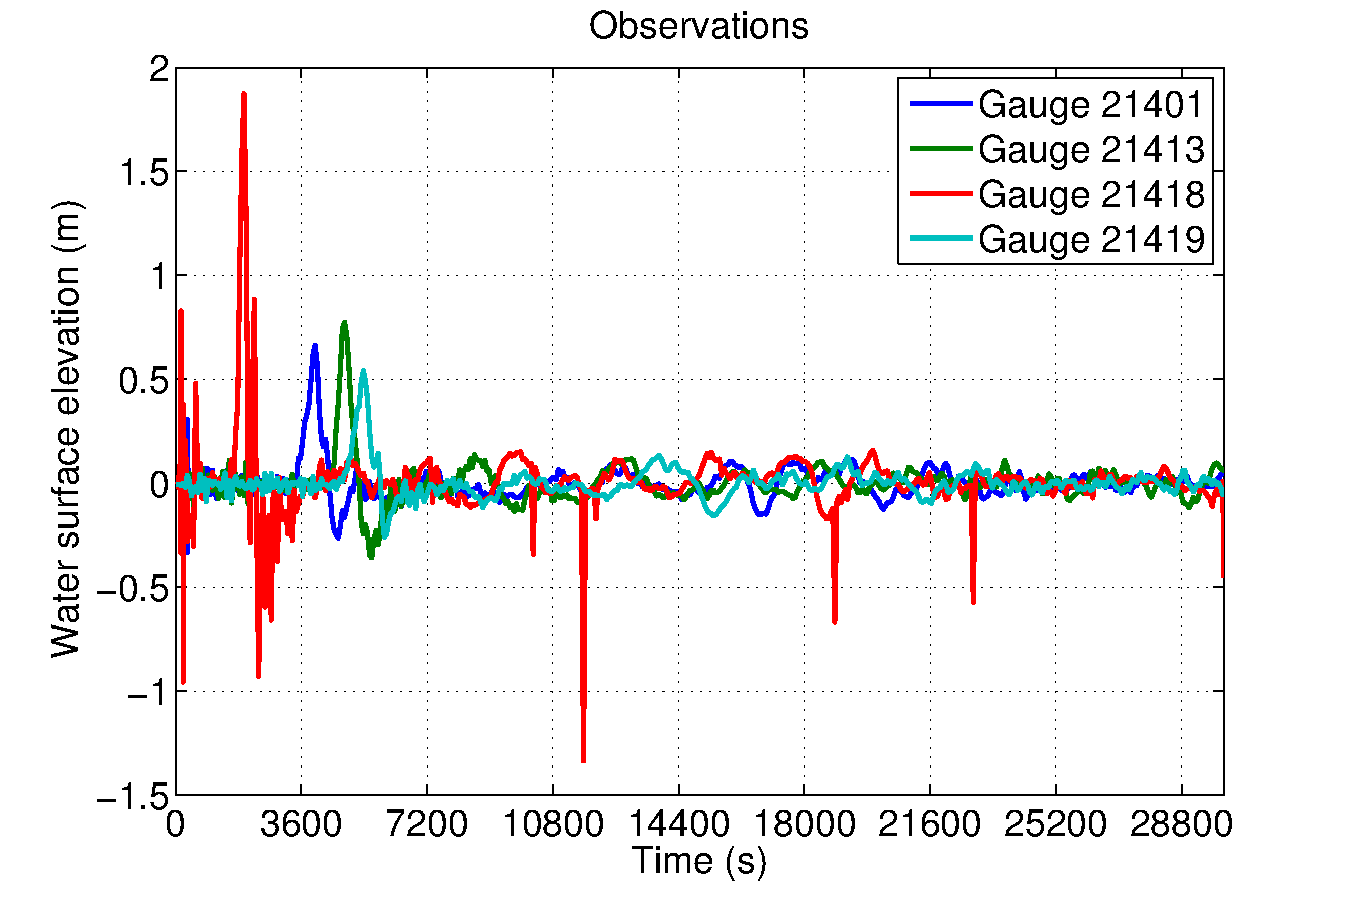
\includegraphics[width=\textwidth]{./figures/obs.pdf} 
    \caption{} \label{fig:setup_buoy_data}
\end{subfigure}
\caption{(a) The topography, bathymetry and gauge locations used in the simulation. (b) Observed de-tided water surface height at all the DART buoys used.}
\label{fig:setup}
\end{figure}

%%%%%%%%%%%%%%%%%%%%%%%%%%%%%%%%%%%%%%%%%%%%%%%%%%%%%%%%%%%%%%%%
\begin{figure}[ht]
\centering
\begin{tabular}{clc}        
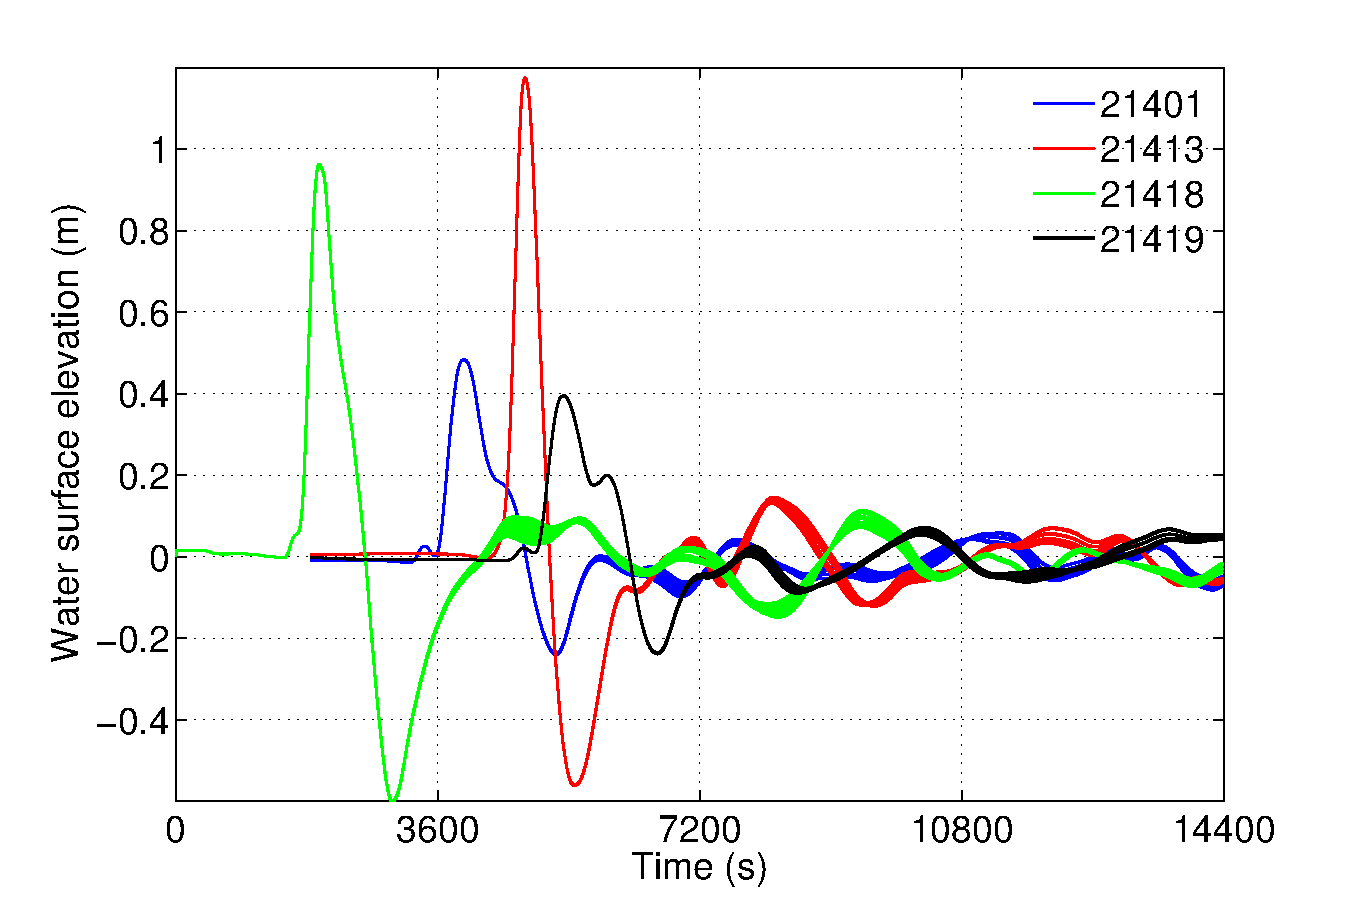
\includegraphics[width=0.6\textwidth]{./figures/rlzs_gauges.pdf} 
\end{tabular}
\caption{125 \geoclaw realizations at different gauge locations.}
\label{fig:rlzs}
\end{figure}
%%%%%%%%%%%%%%%%%%%%%%%%%%%%%%%%%%%%%%%%%%%%%%%%%%%%%%%%%%%%%%%%

\begin{figure}[ht]
\centering
\begin{tabular}{clc}        
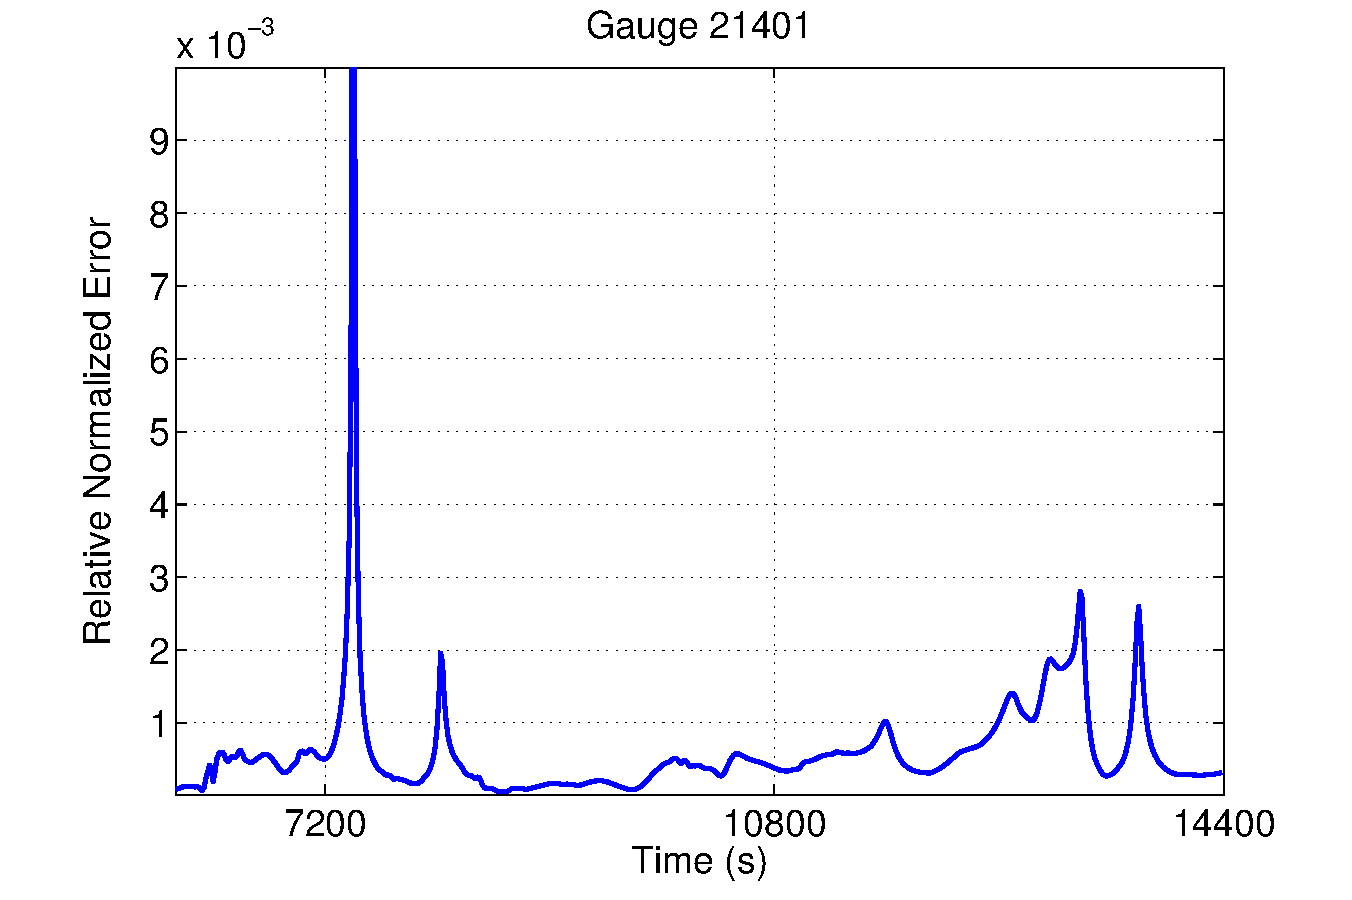
\includegraphics[width=0.5\textwidth]{./figures/error_gauge1.pdf} &
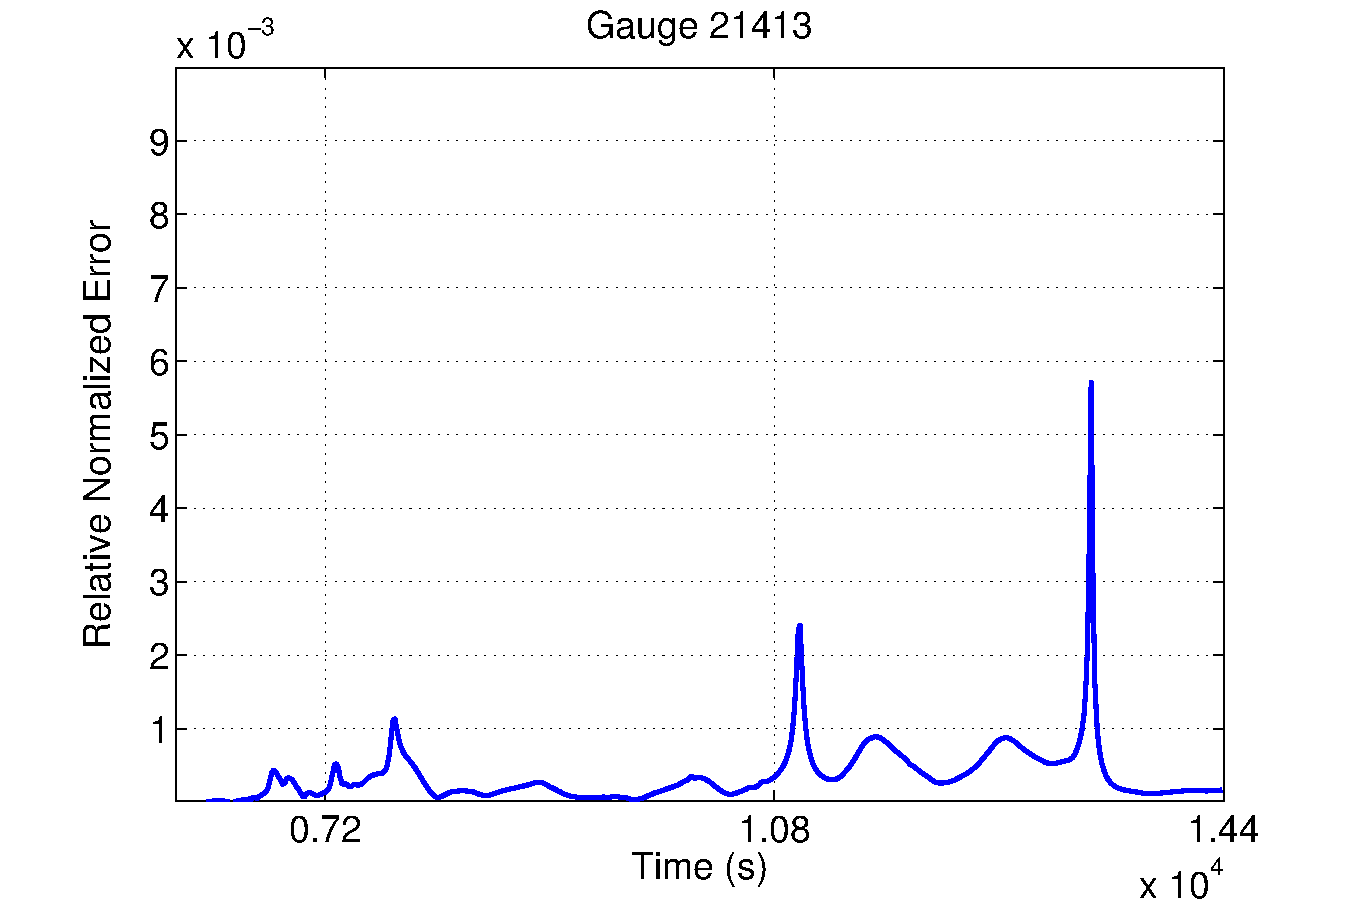
\includegraphics[width=0.5\textwidth]{./figures/error_gauge2.pdf} \\
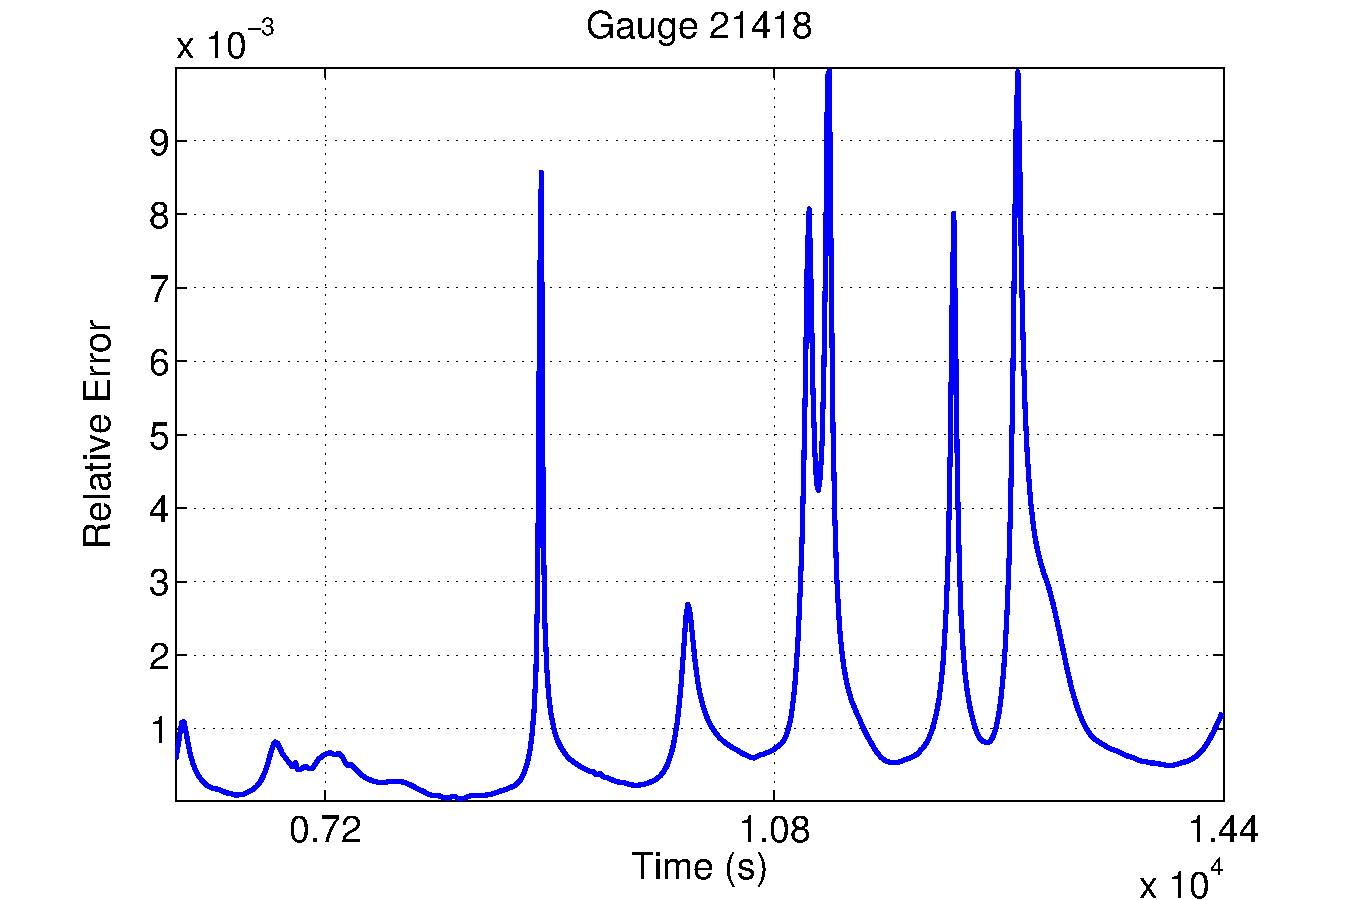
\includegraphics[width=0.5\textwidth]{./figures/error_gauge3.pdf} &
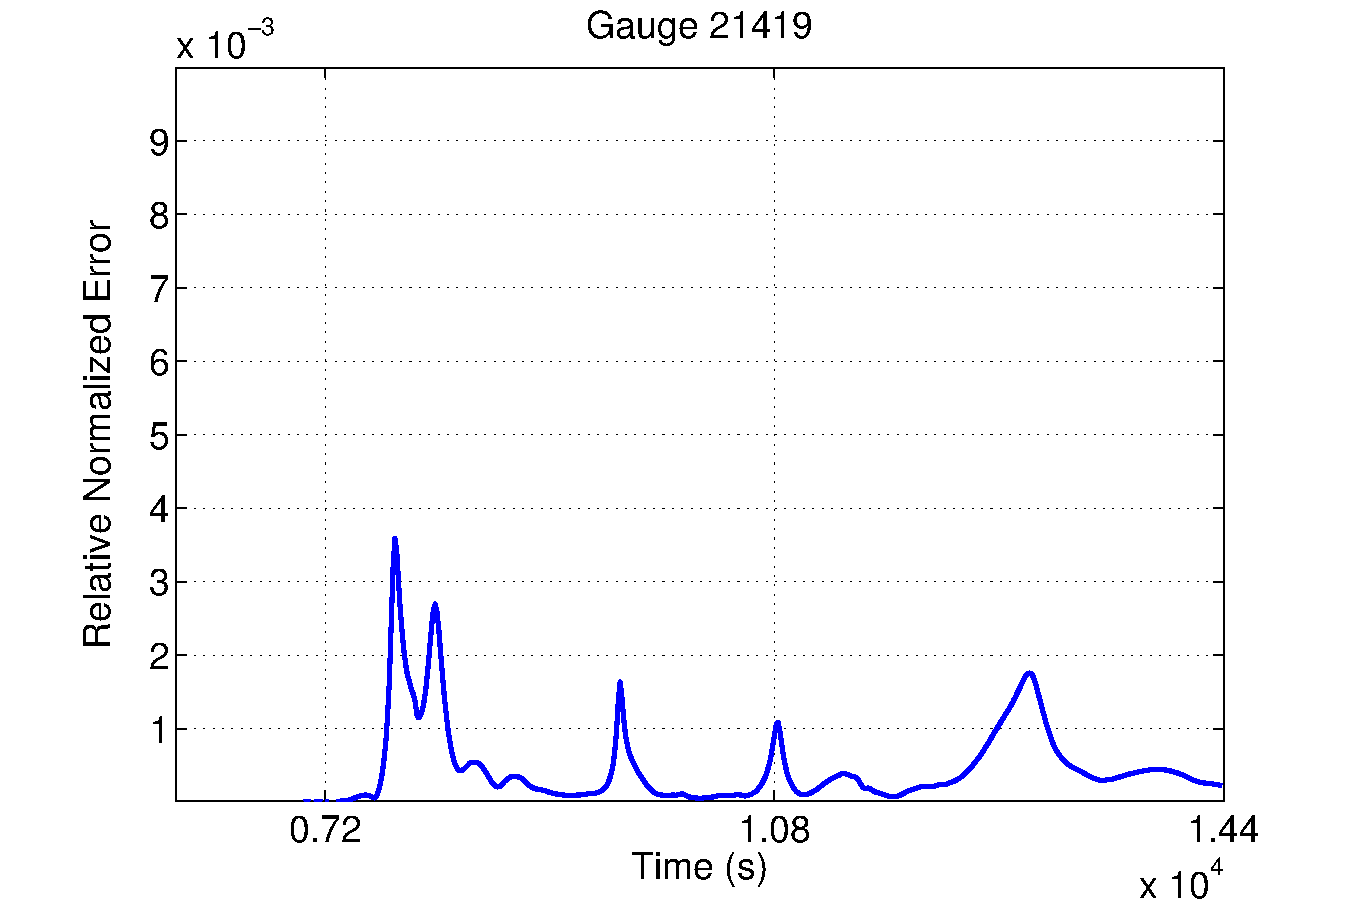
\includegraphics[width=0.5\textwidth]{./figures/error_gauge4.pdf} 

\end{tabular}
\caption{Relative normalized error between realizations and 
the corresponding PC surrogates at different gauge locations
calculated using Equation~(\ref{eq:error}).}
\label{fig:error}
\end{figure}   
%%%%%%%%%%%%%%%%%%%%%%%%%%%%%%%%%%%%%%%%%%%%%%%%%%%%%%%%%%%%%%%%
\begin{figure}[ht]
\centering

\begin{tabular}{clcl}
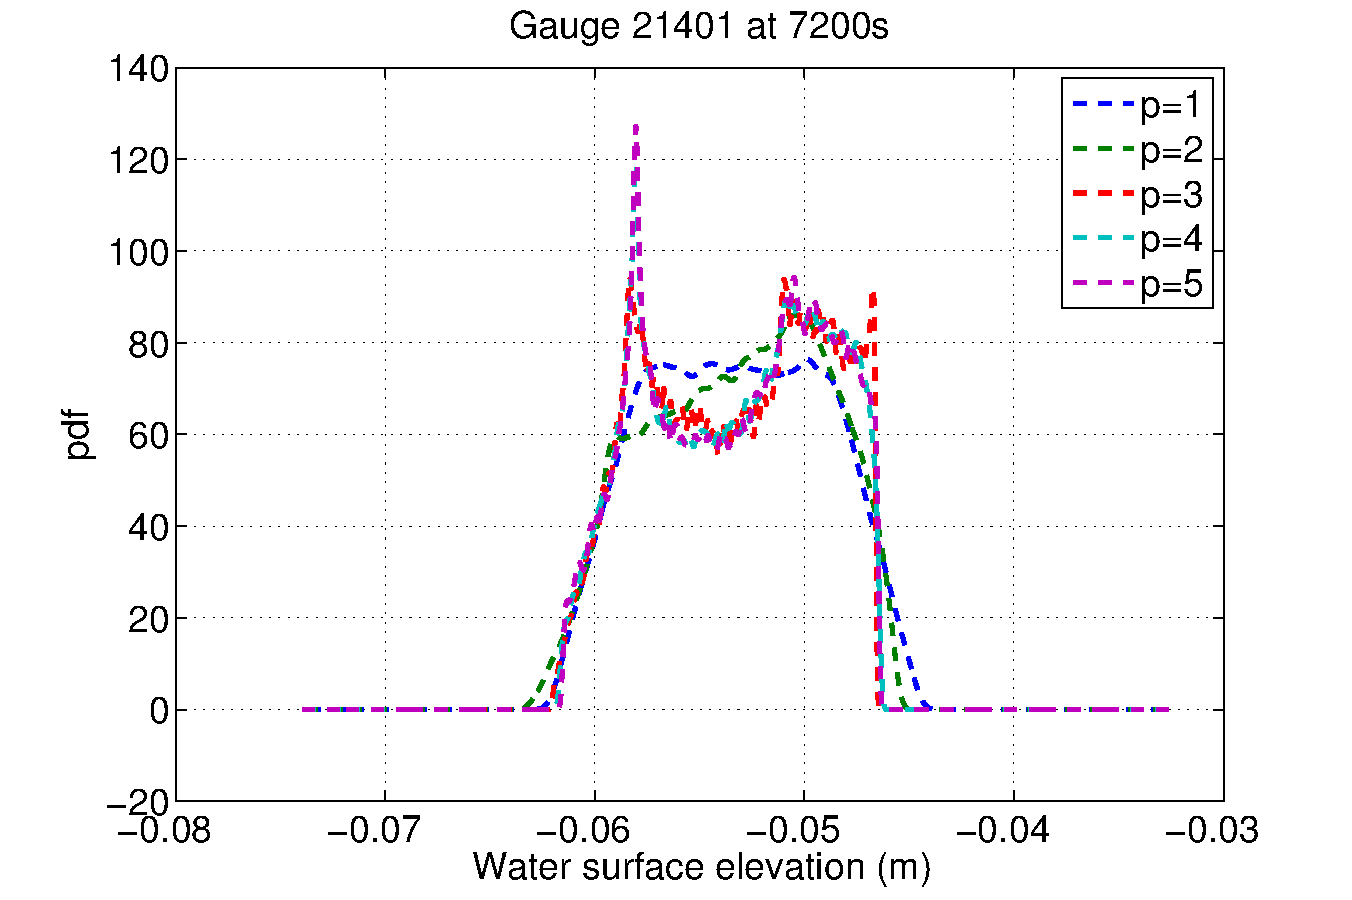
\includegraphics[width=0.5\textwidth]{./figures/pdfs1_2.pdf} &
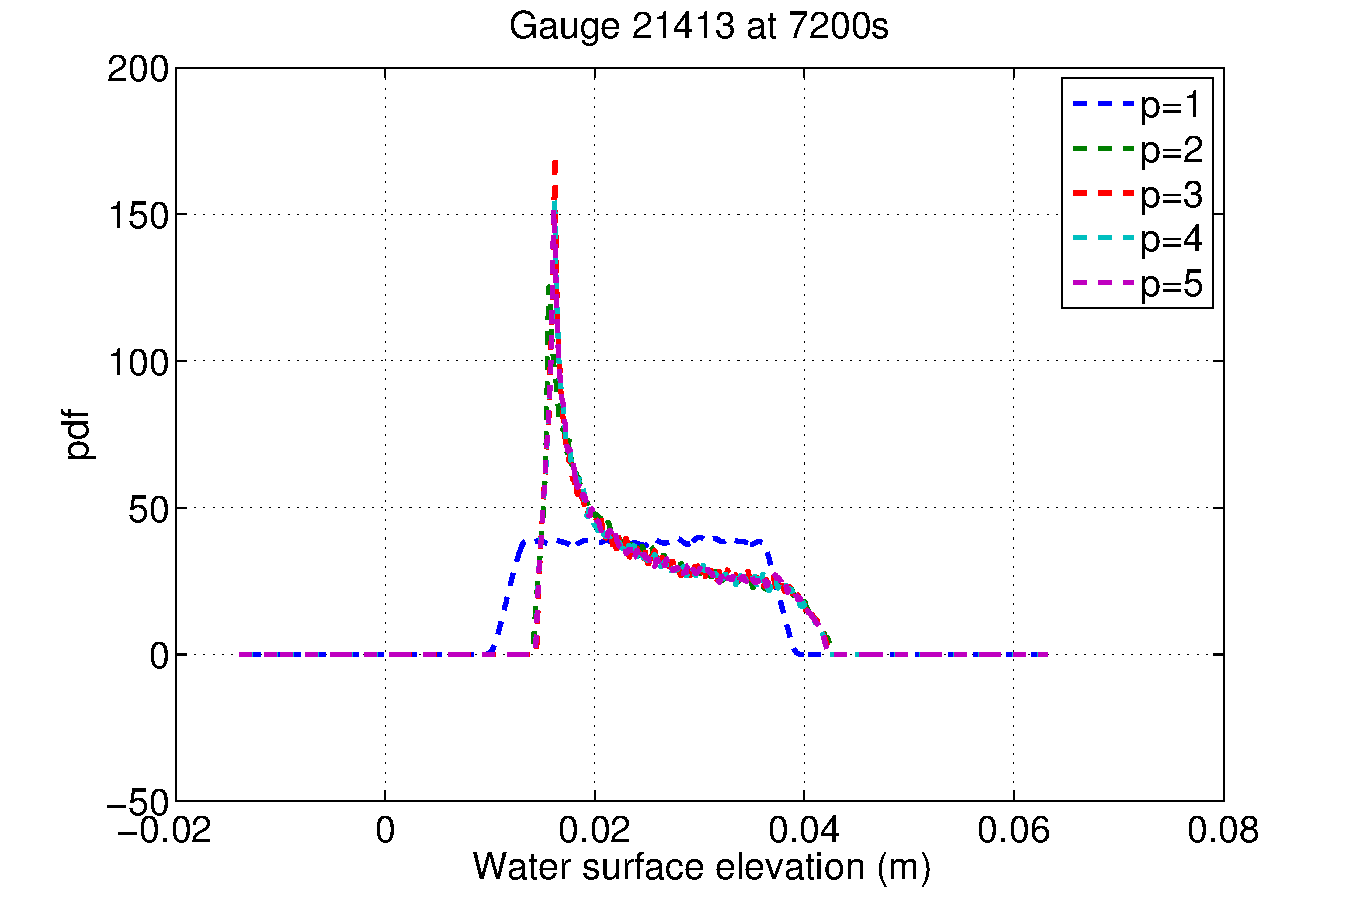
\includegraphics[width=0.5\textwidth]{./figures/pdfs2_2.pdf} \\
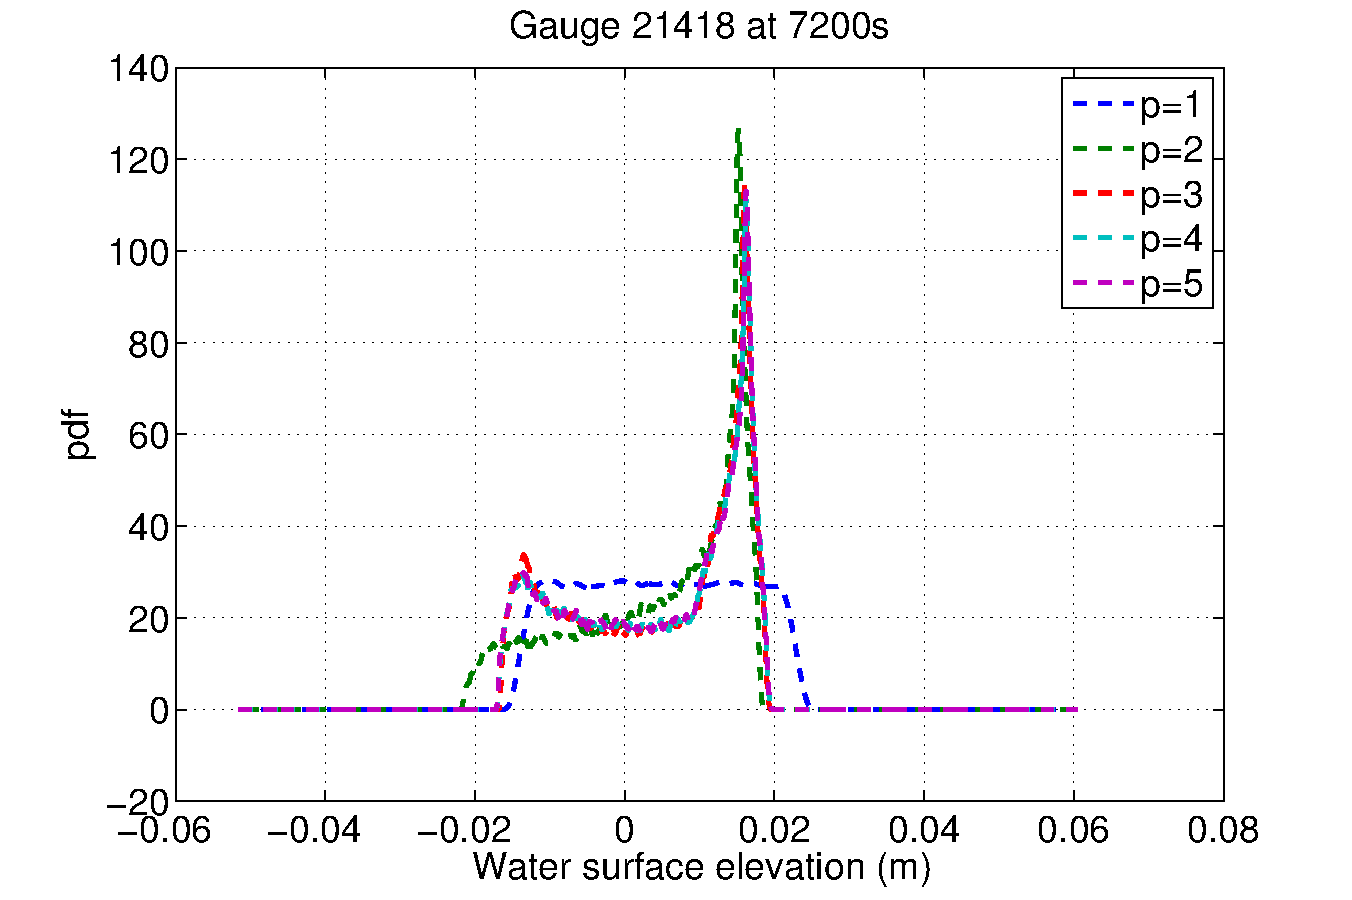
\includegraphics[width=0.5\textwidth]{./figures/pdfs3_2.pdf} &
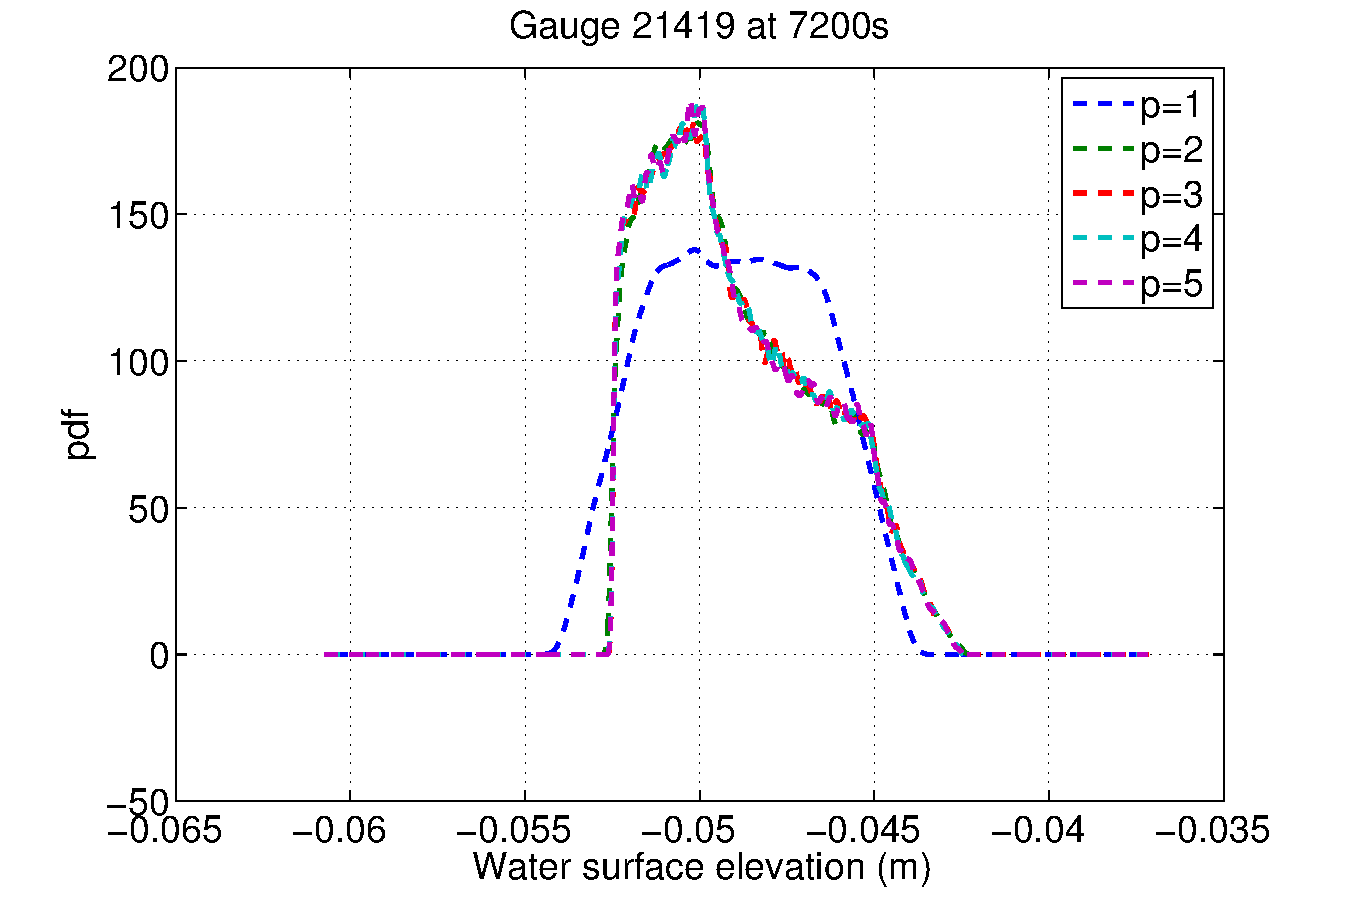
\includegraphics[width=0.5\textwidth]{./figures/pdfs4_2.pdf}
\end{tabular}
\caption{pdf of water surface elevation at the different gauge locations at t = 7200 s.}
\label{fig:pdfs2}
\end{figure}
%%%%%%%%%%%%%%%%%%%%%%%%%%%%%%%%%%%%%%%%%%%%%%%%%%%%%%%%%%%%%%%%
\begin{figure}[ht]
\centering
\begin{tabular}{clc}
        
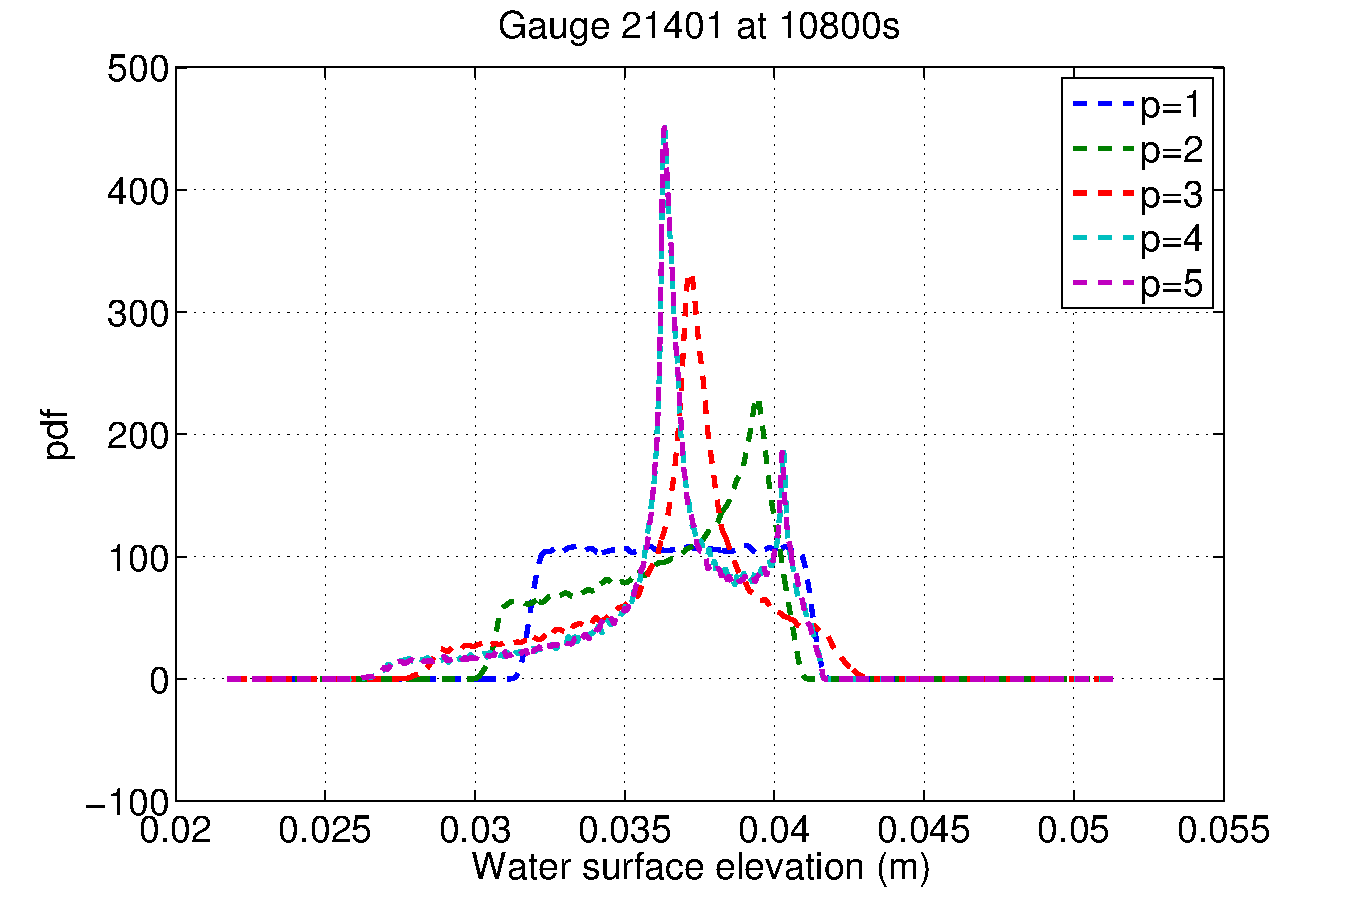
\includegraphics[width=0.5\textwidth]{./figures/pdfs1_3.pdf} &
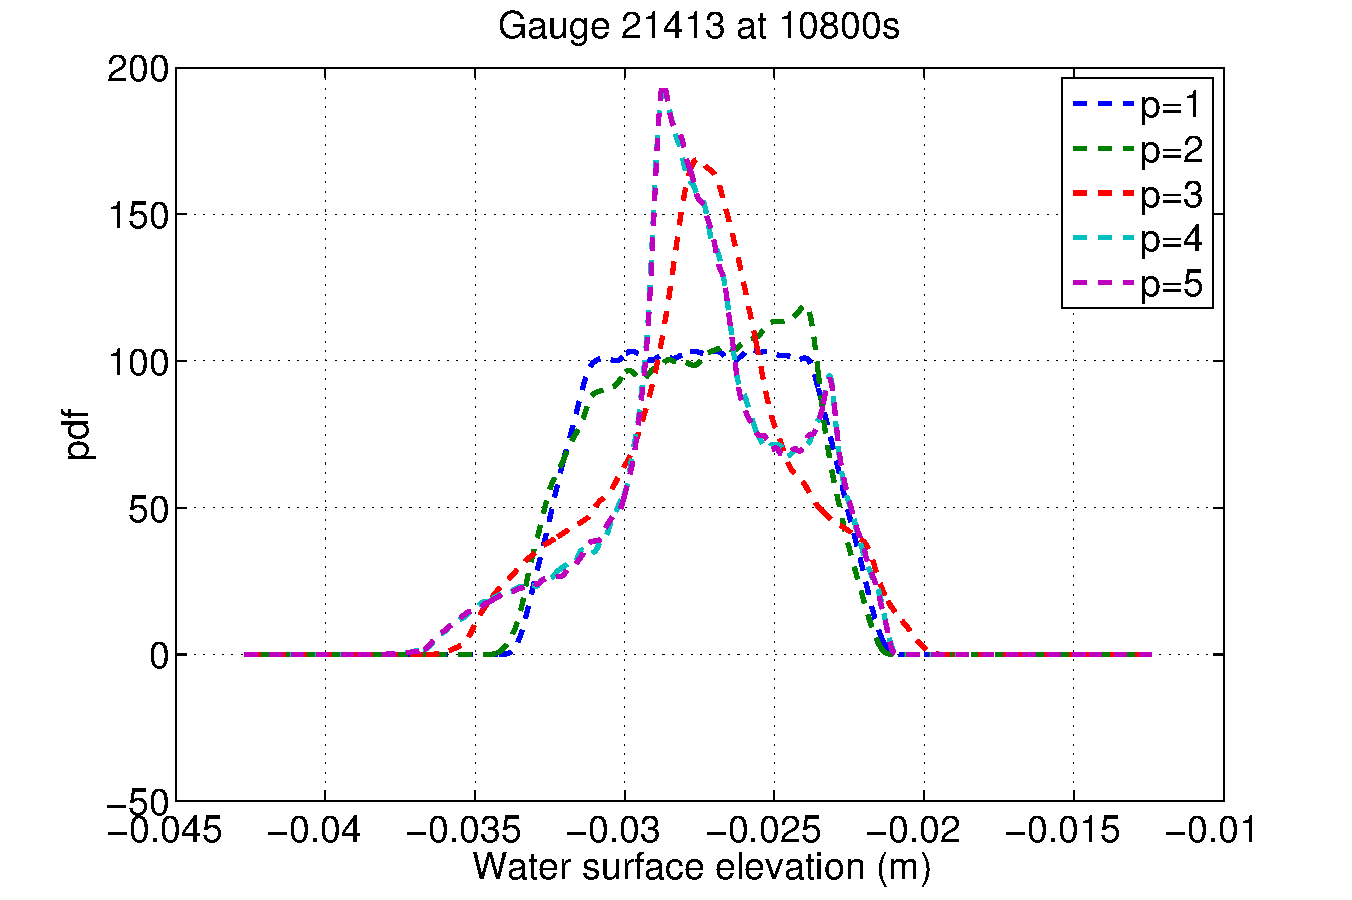
\includegraphics[width=0.5\textwidth]{./figures/pdfs2_3.pdf} \\
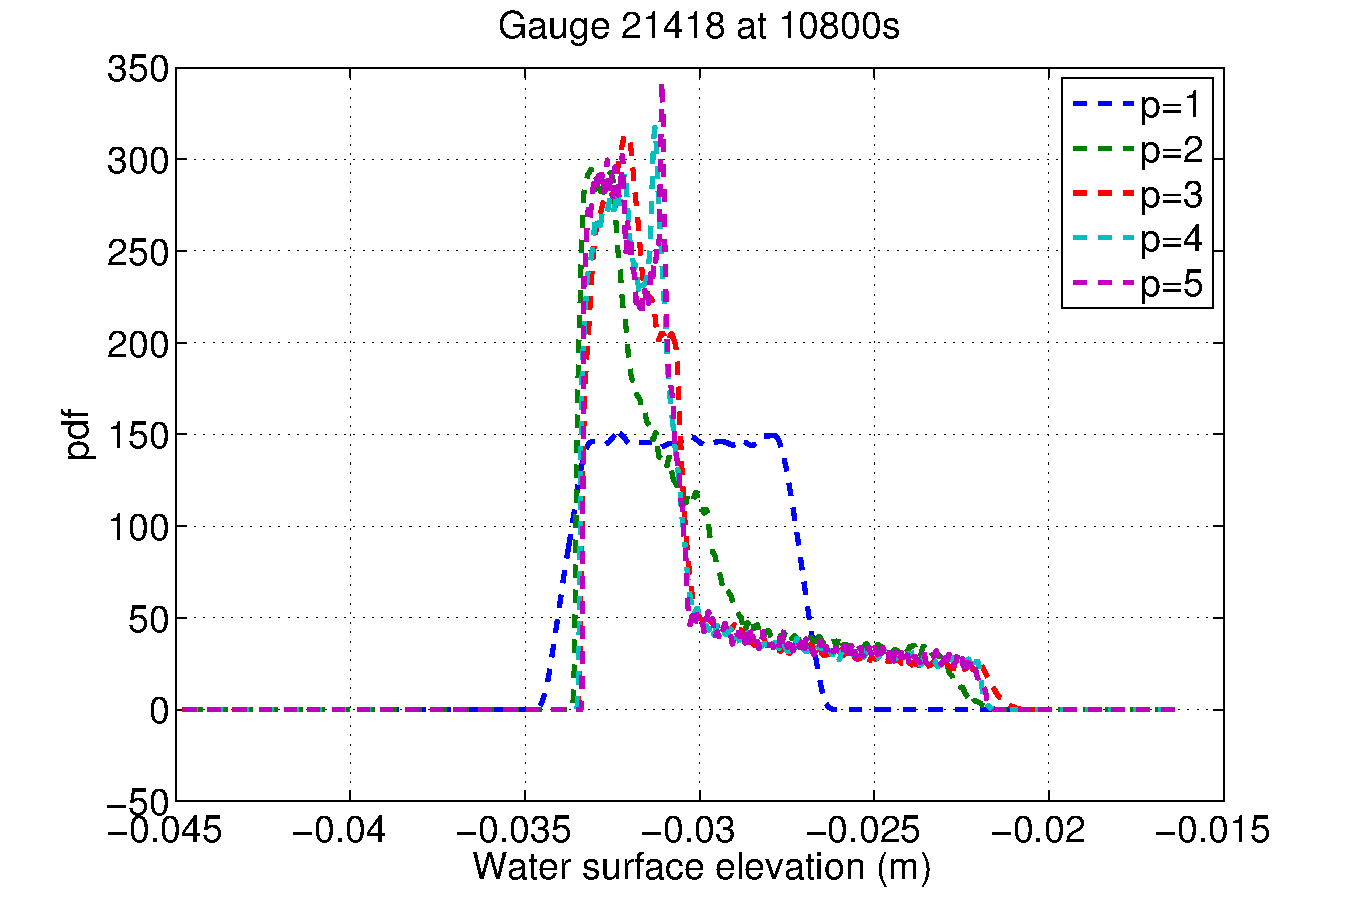
\includegraphics[width=0.5\textwidth]{./figures/pdfs3_3.pdf} &
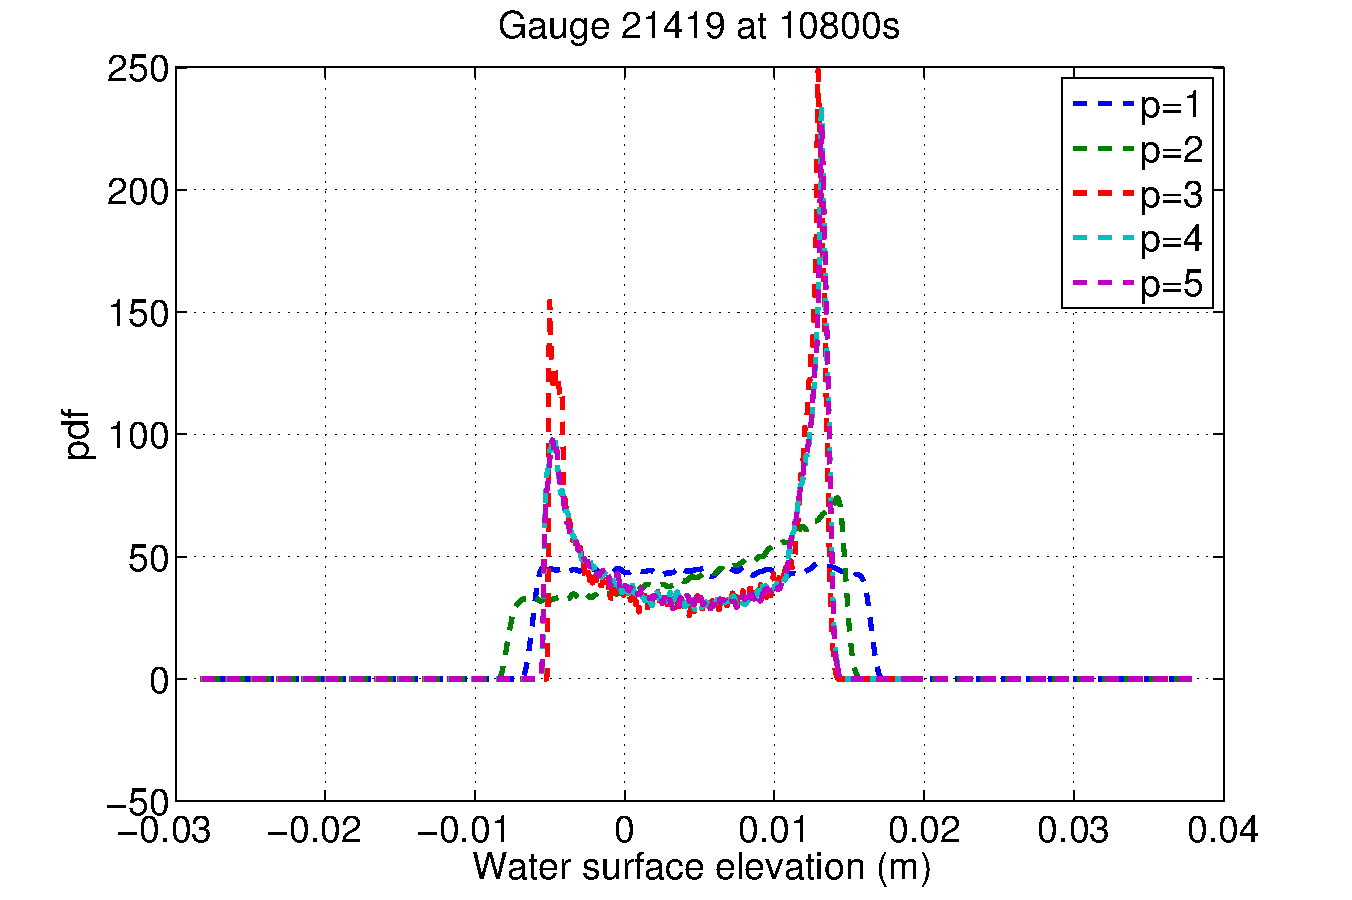
\includegraphics[width=0.5\textwidth]{./figures/pdfs4_3.pdf}
\end{tabular}
\caption{pdf of water surface elevation at the different gauge locations at t = 10800 s.}
\label{fig:pdfs3}
\end{figure}
%%%%%%%%%%%%%%%%%%%%%%%%%%%%%%%%%%%%%%%%%%%%%%%%%%%%%%%%%%%%%%%%
\begin{figure}[ht]
\begin{tabular}{clc}
        
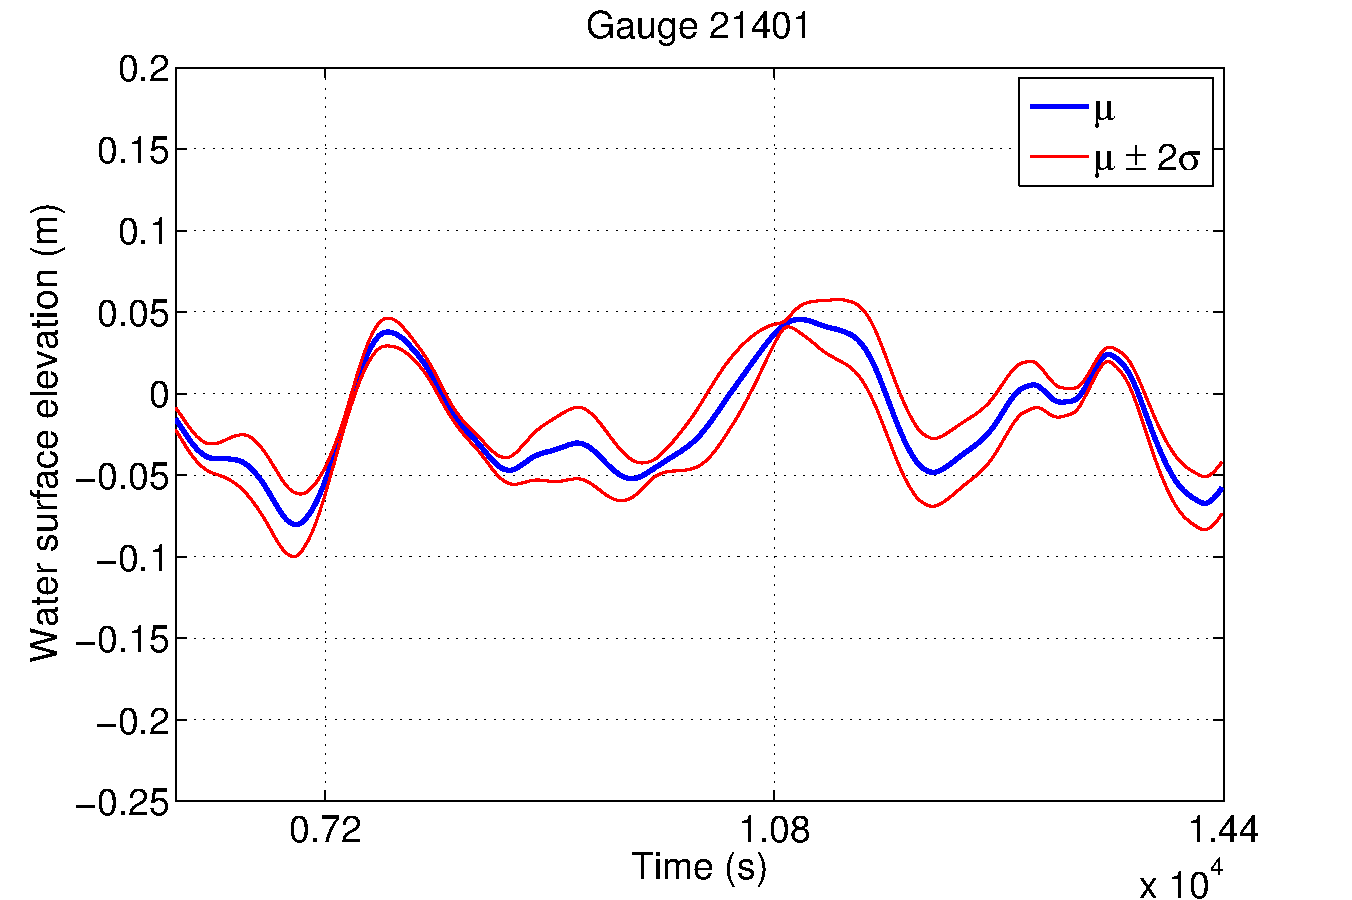
\includegraphics[width=0.475\textwidth]{./figures/musigma1.pdf} &
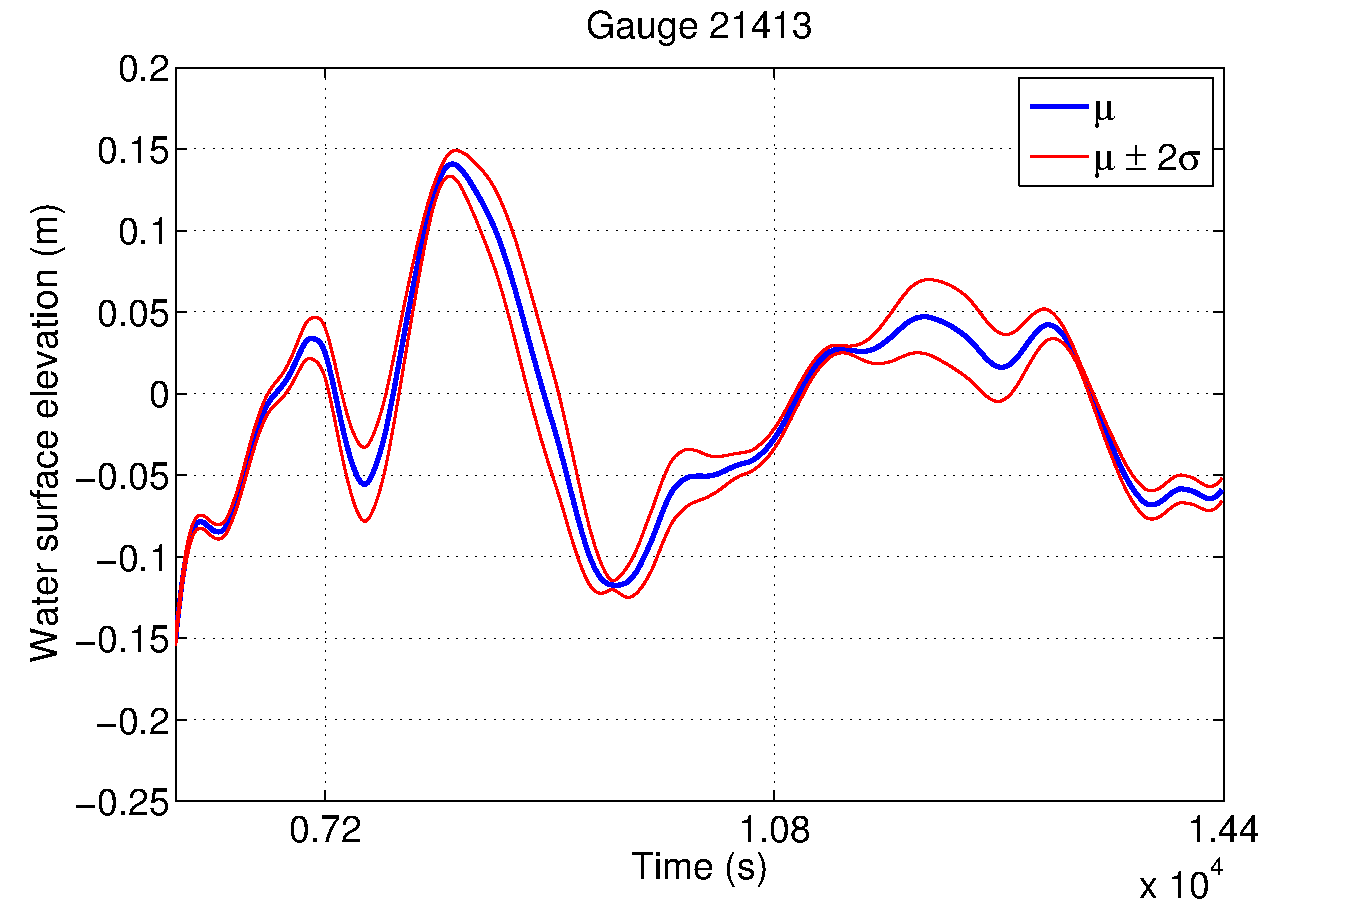
\includegraphics[width=0.475\textwidth]{./figures/musigma2.pdf} \\
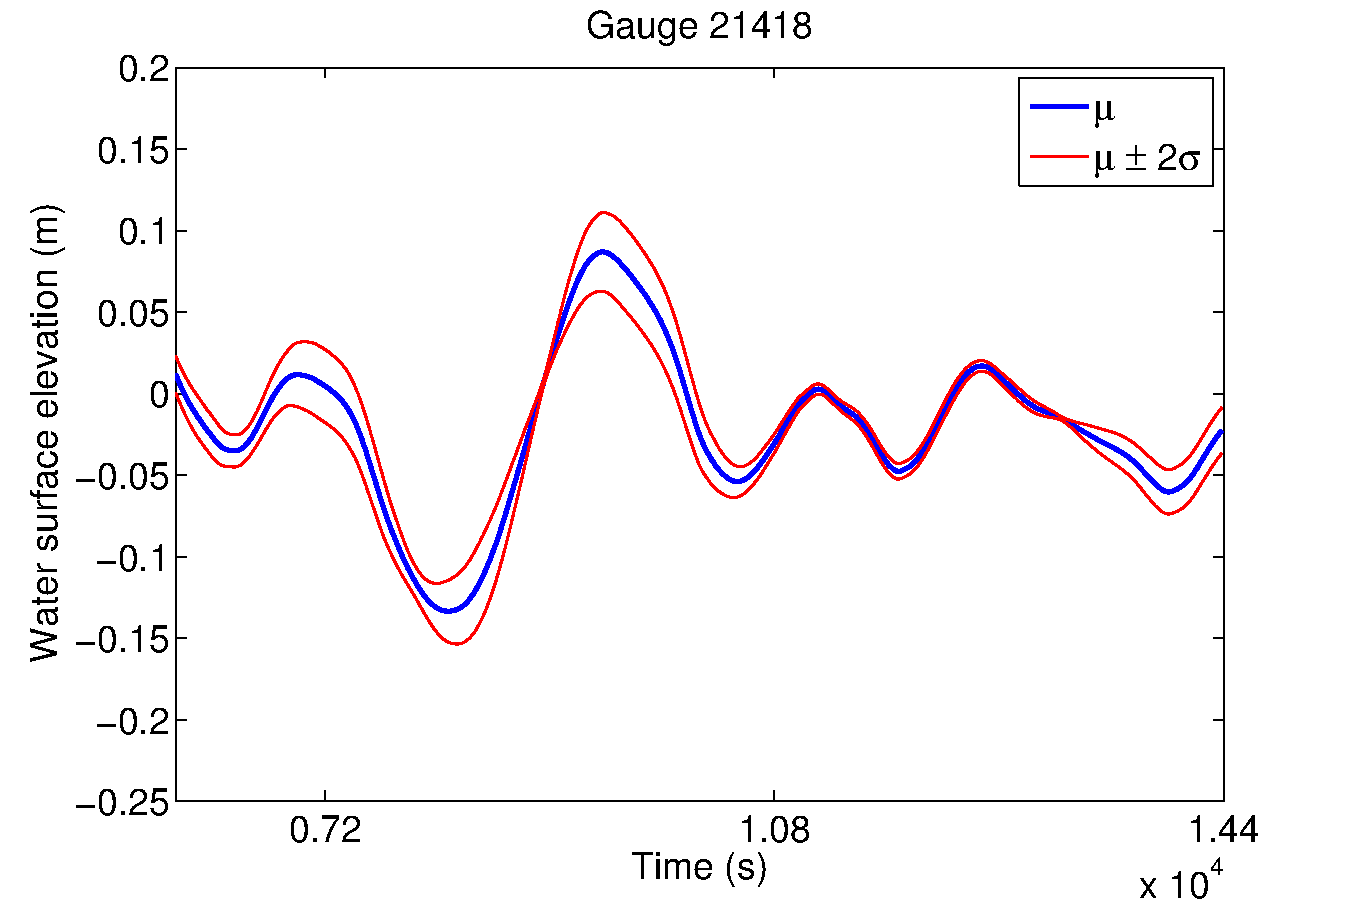
\includegraphics[width=0.475\textwidth]{./figures/musigma3.pdf} &
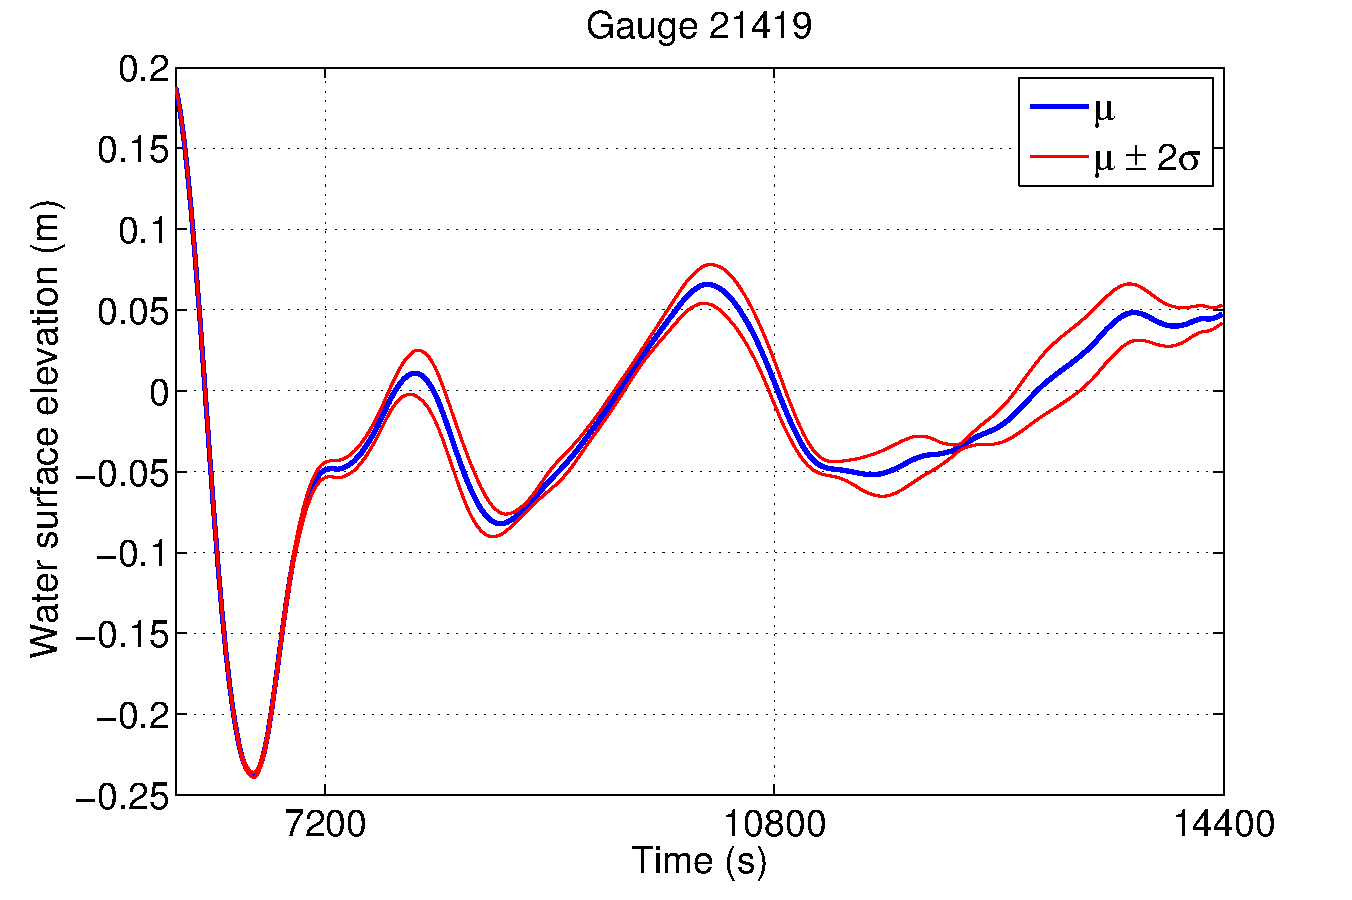
\includegraphics[width=0.475\textwidth]{./figures/musigma4.pdf}
\end{tabular}
\caption{Evolution of PC mean water surface elevation at different gauge locations.}
\label{fig:ave}
\end{figure}
%%%%%%%%%%%%%%%%%%%%%%%%%%%%%%%%%%%%%%%%%%%%%%%%%%%%%%%%%%%%%%%%
\begin{figure}[ht]
\begin{tabular}{clc}
%        
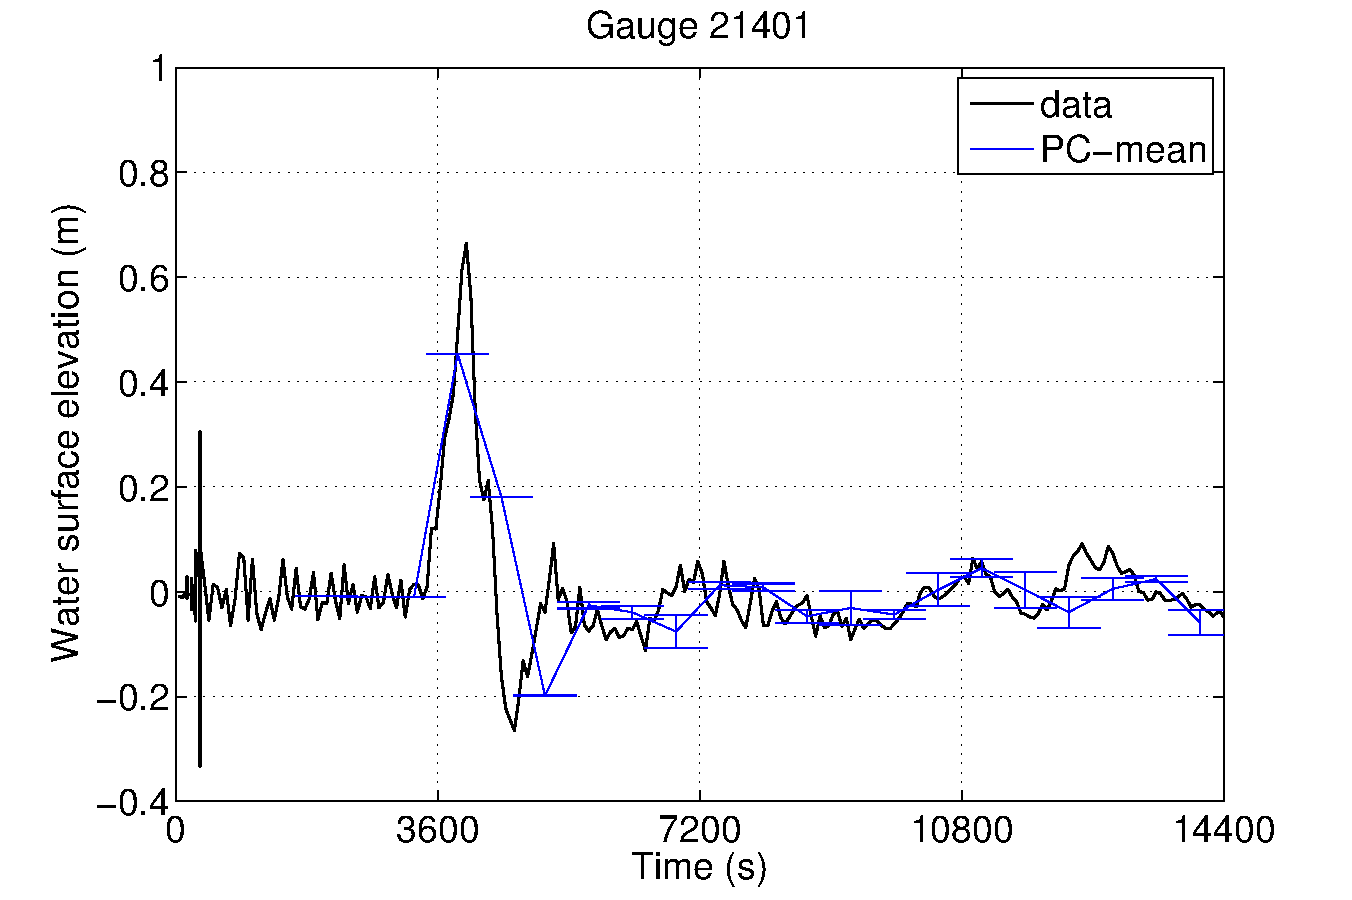
\includegraphics[width=0.475\textwidth]{./figures/compare1.pdf} &
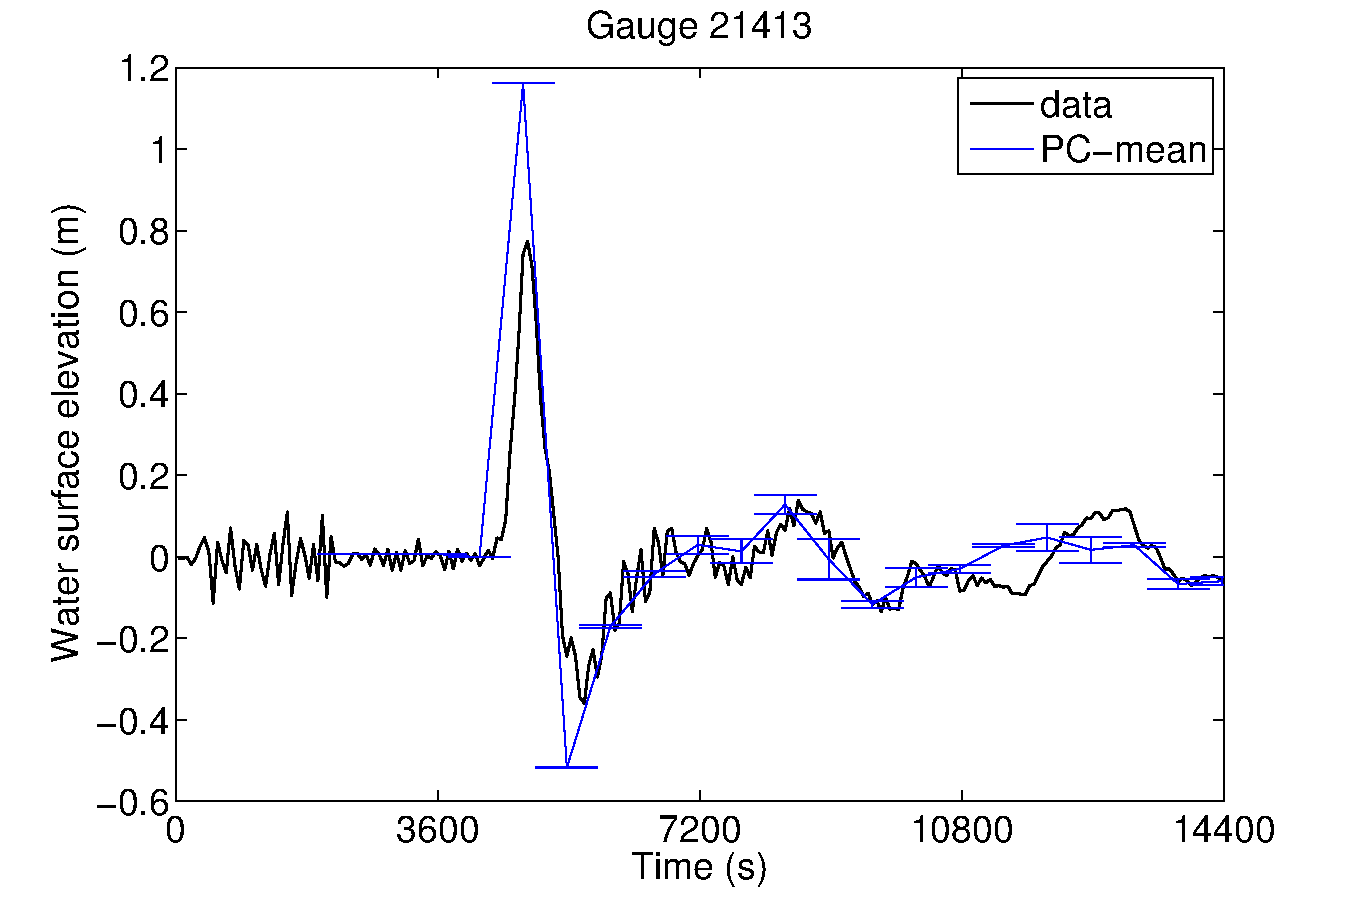
\includegraphics[width=0.475\textwidth]{./figures/compare2.pdf} \\
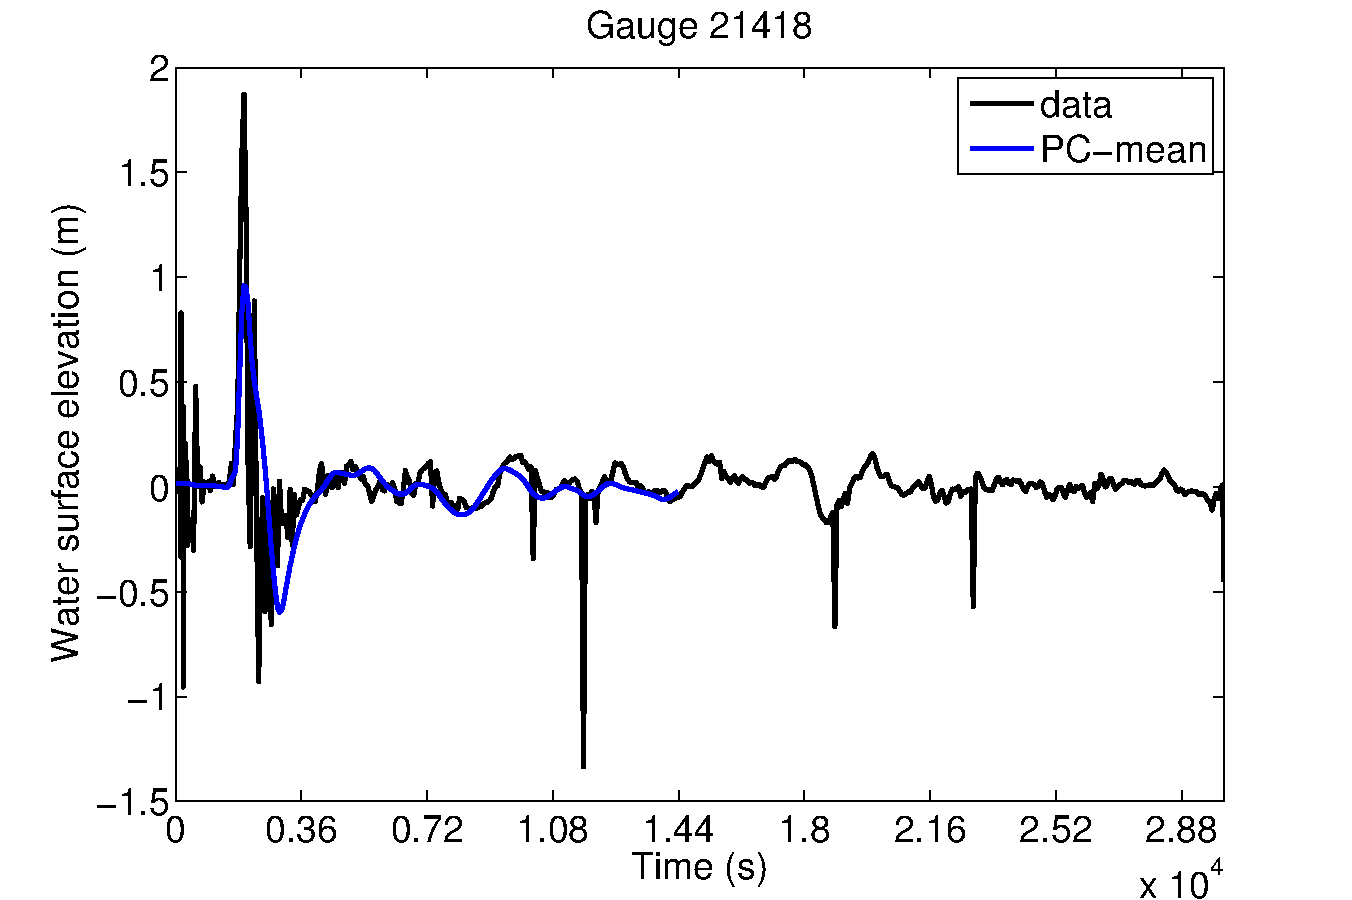
\includegraphics[width=0.475\textwidth]{./figures/compare3.pdf} &
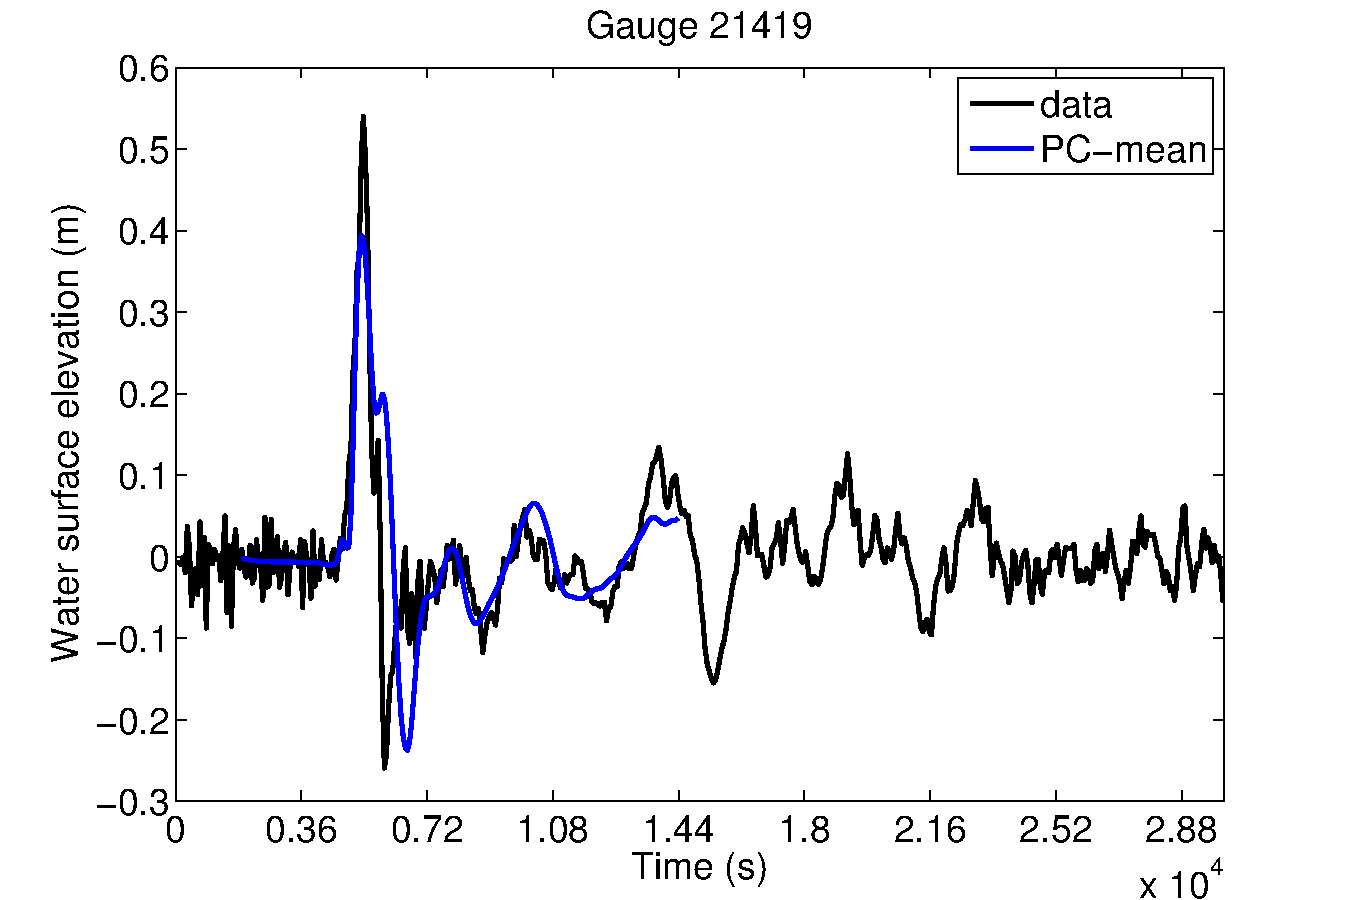
\includegraphics[width=0.475\textwidth]{./figures/compare4.pdf}
\end{tabular}
\caption{Comparison of PC mean 
and observed data of water surface elevation with time at the four gauges.}
\label{fig:compare}
\end{figure}  
%%%%%%%%%%%%%%%%%%%%%%%%%%%%%%%%%%%%%%%%%%%%%%%%%%%%%%%%%%%%%%%%
\begin{figure}[ht]
        \begin{tabular}{ccc}
\hspace*{-55pt}
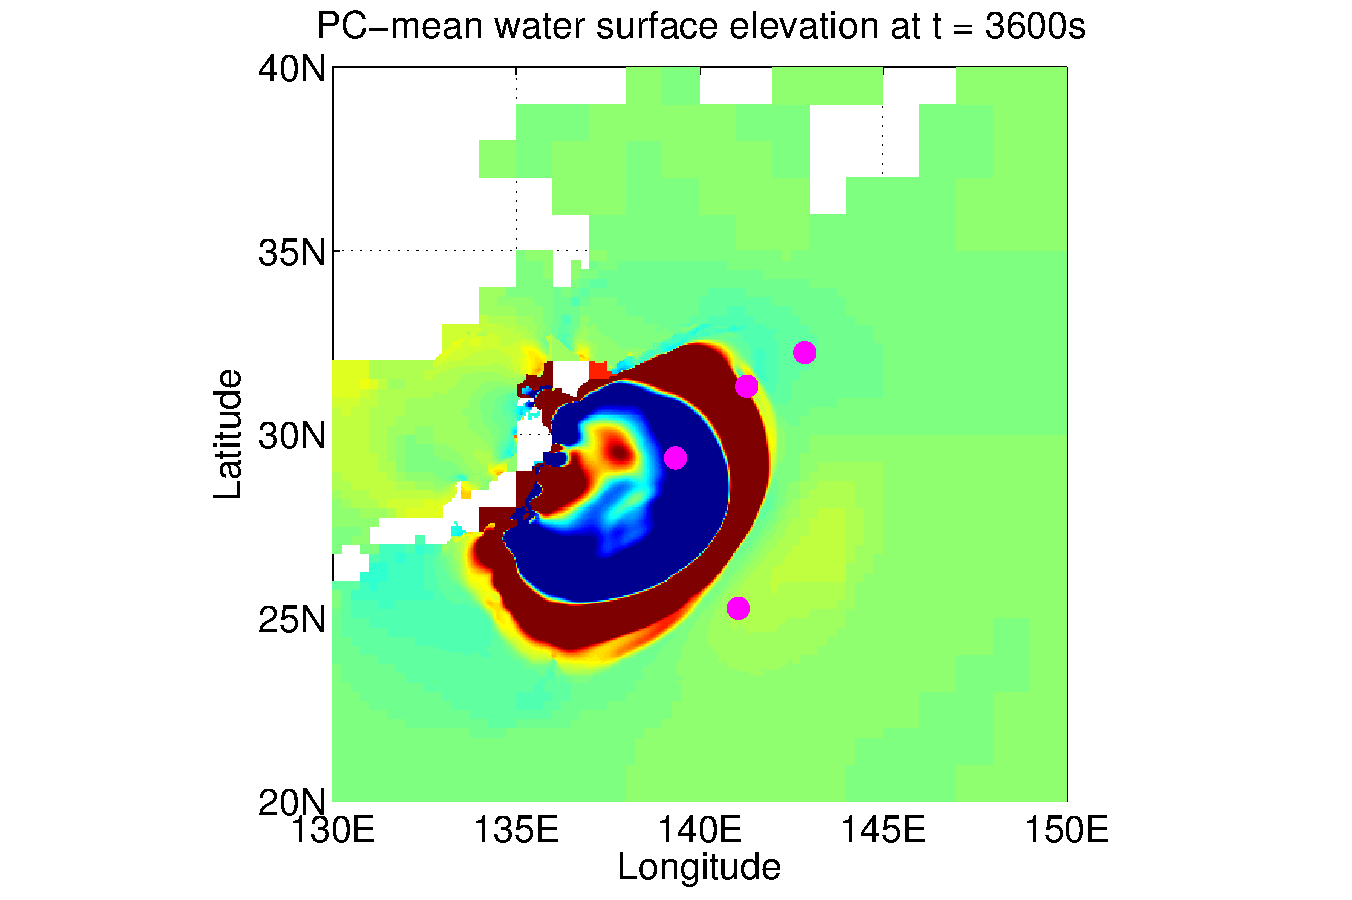
\includegraphics[width=0.45\textwidth]{./figures/mean2d1.pdf} &
\hspace*{-45pt}
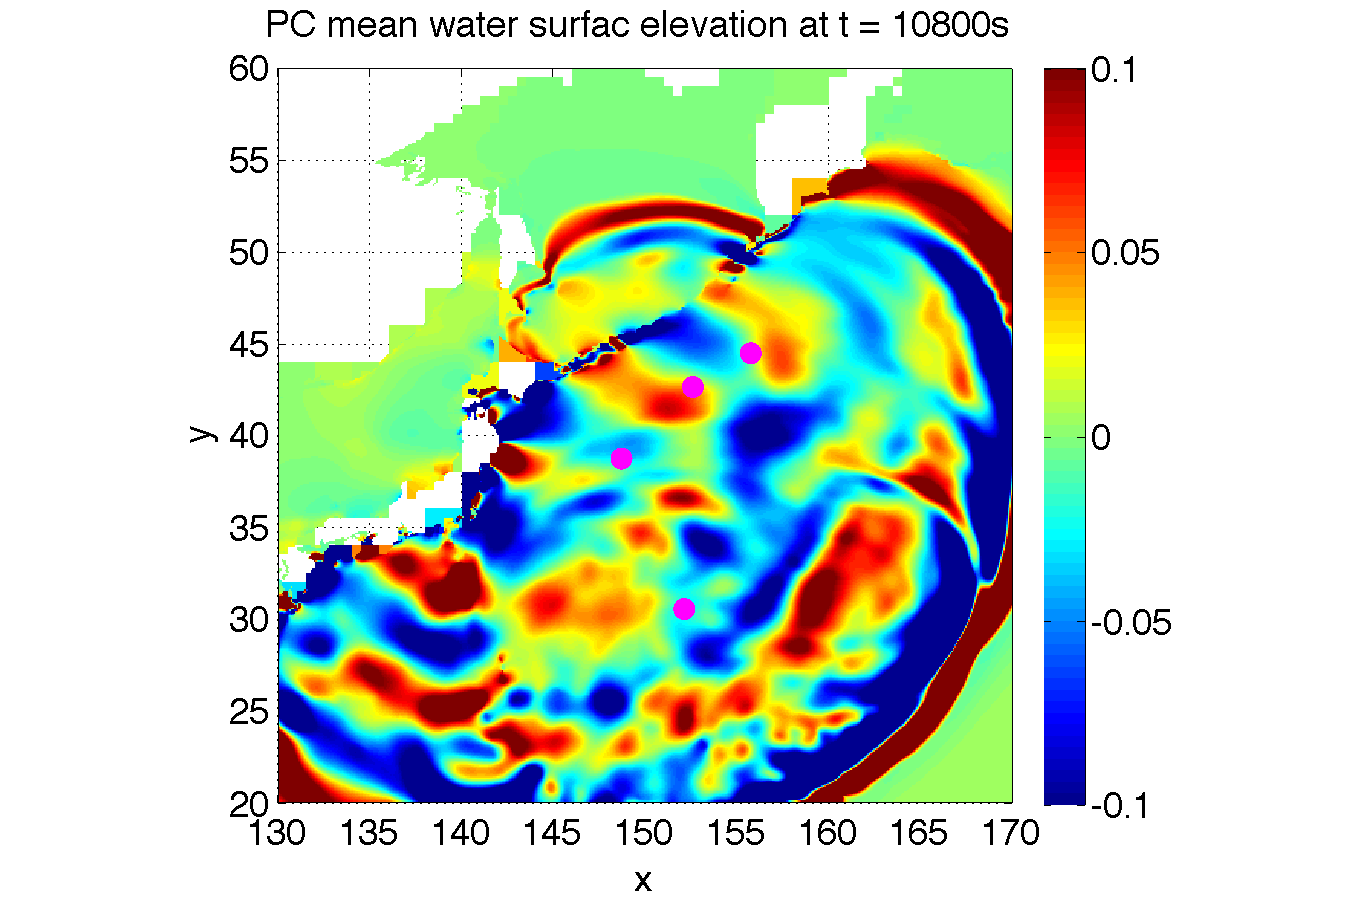
\includegraphics[width=0.45\textwidth]{./figures/mean2d3.pdf} &
\hspace*{-45pt}
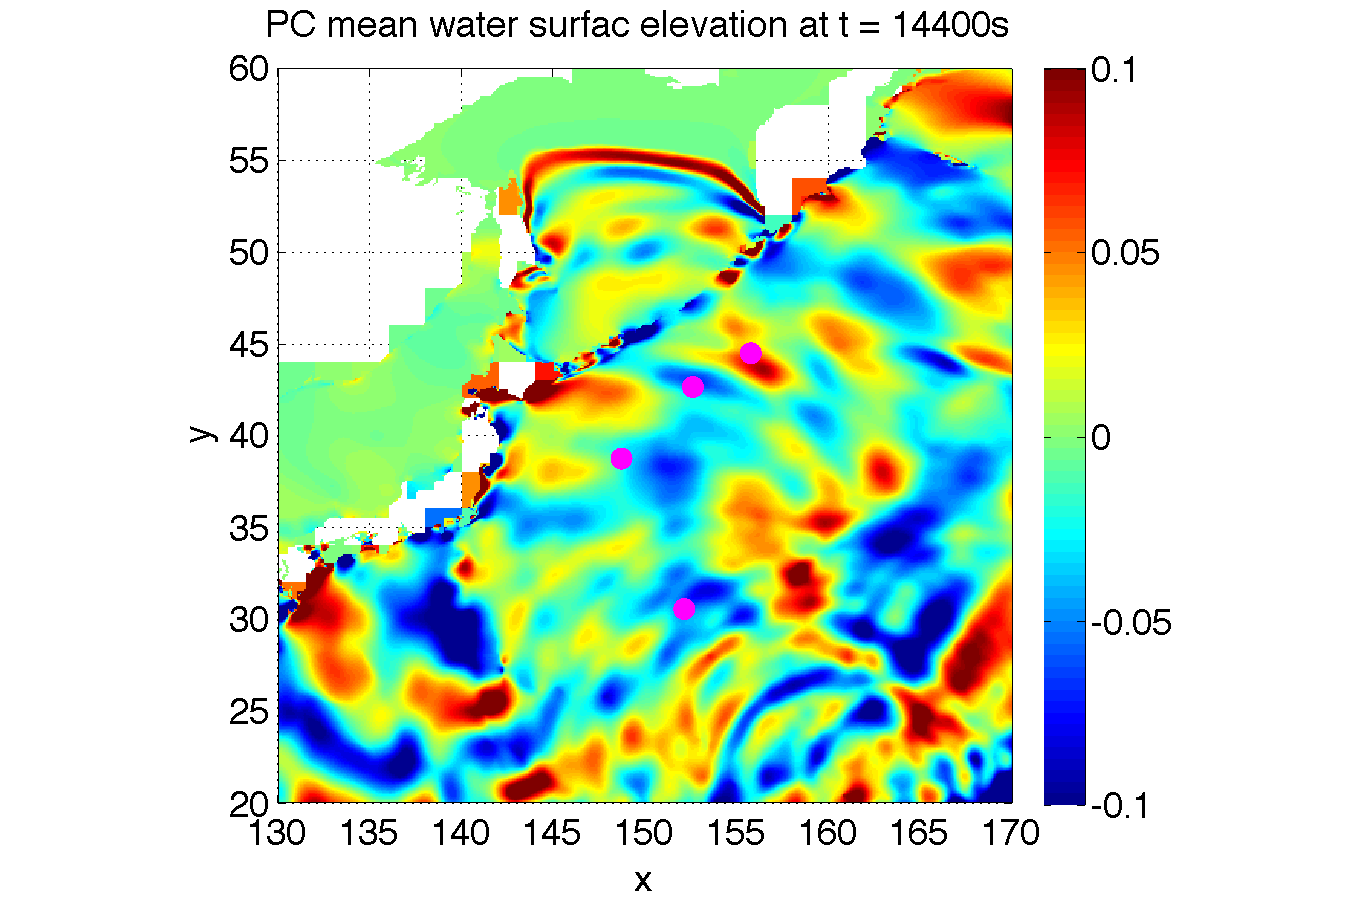
\includegraphics[width=0.45\textwidth]{./figures/mean2d4.pdf} \\
\hspace*{-55pt}
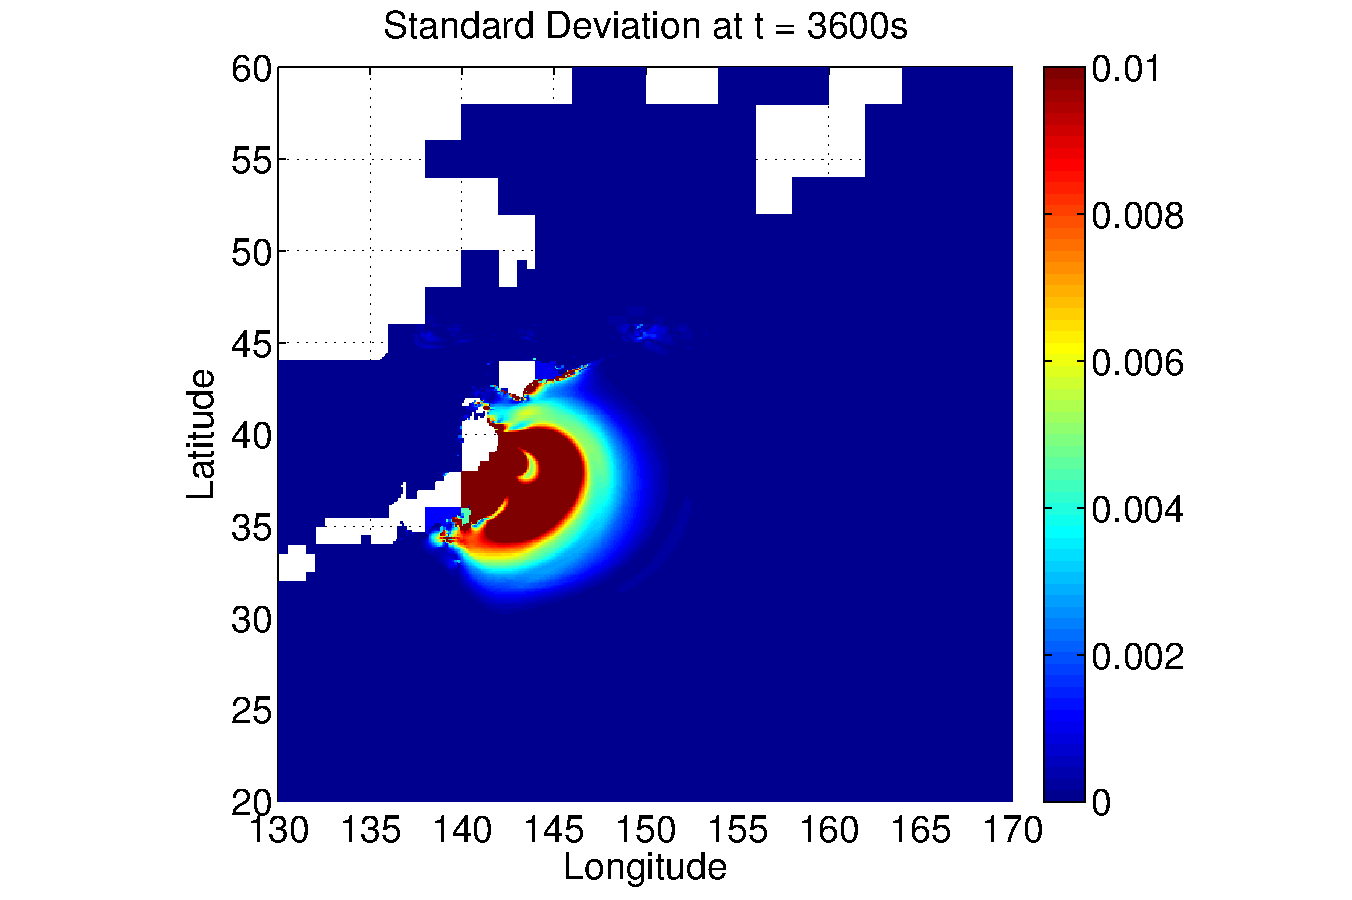
\includegraphics[width=0.45\textwidth]{./figures/sigma2d1.pdf} &
\hspace*{-45pt}
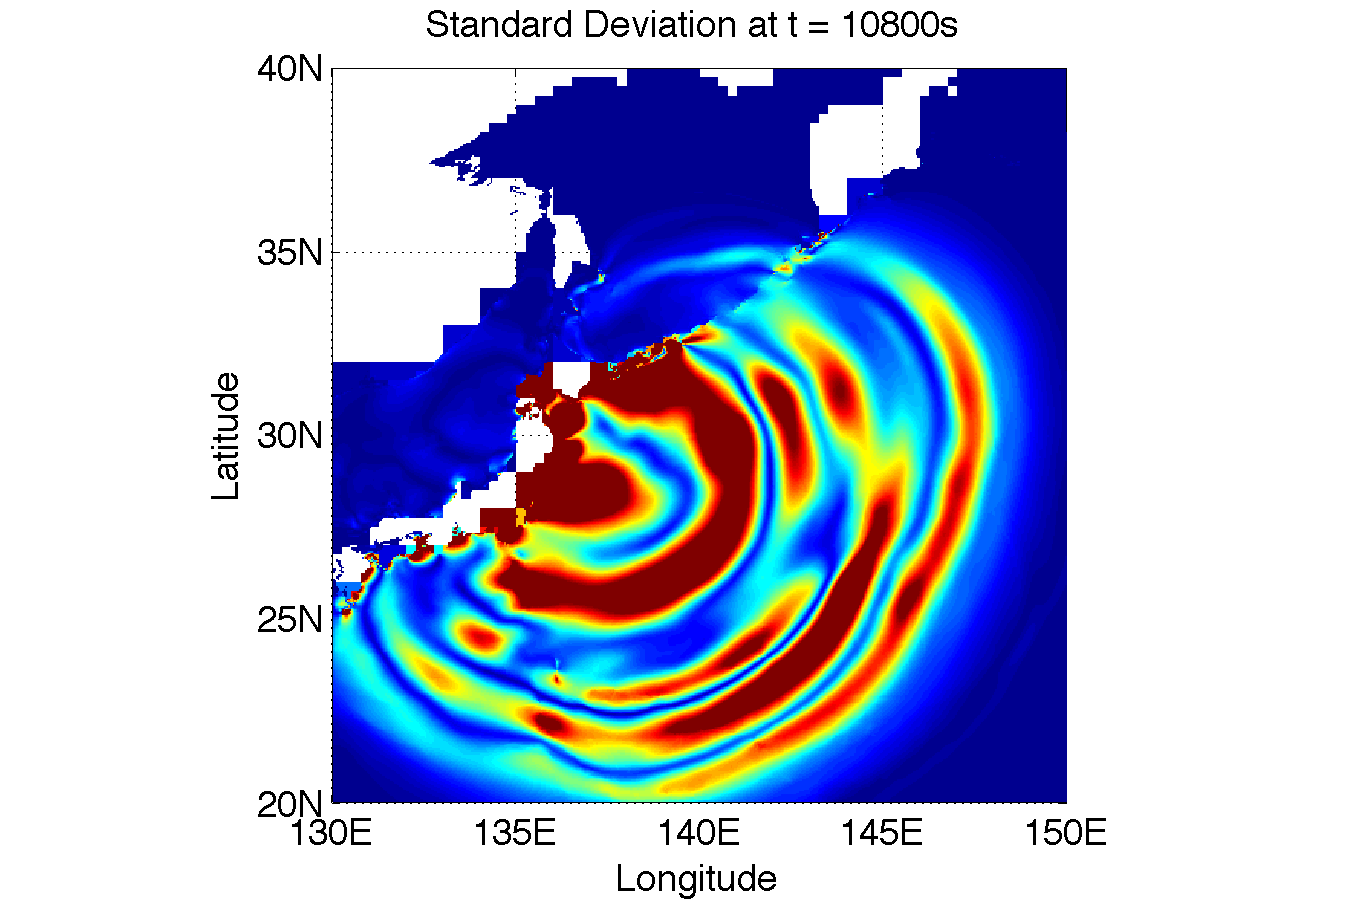
\includegraphics[width=0.45\textwidth]{./figures/sigma2d3.pdf} &
\hspace*{-45pt}
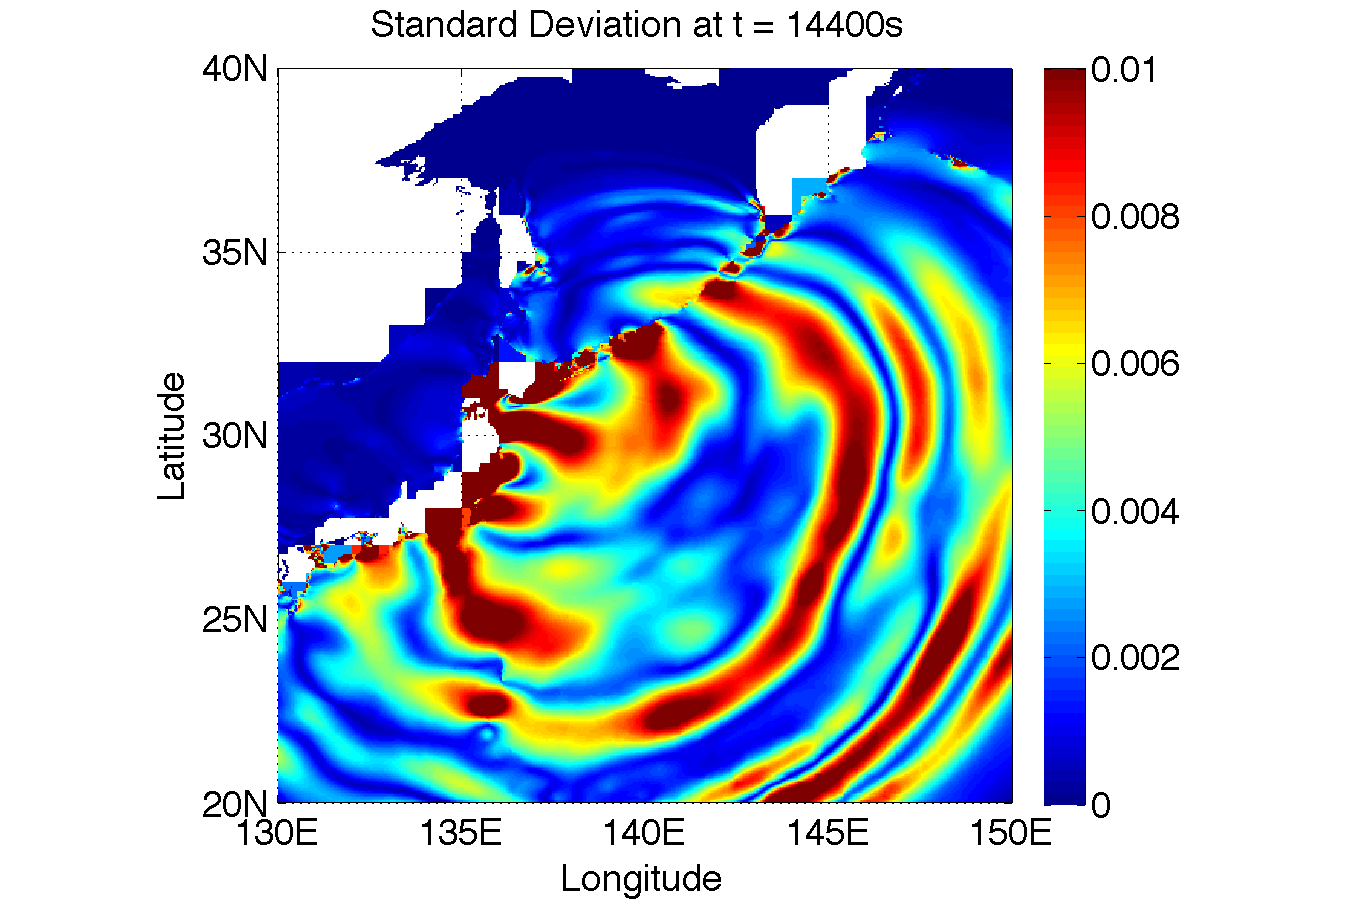
\includegraphics[width=0.45\textwidth]{./figures/sigma2d4.pdf}
\end{tabular}
\caption{PC mean (top row) and standard deviation (bottom row) of the water surface elevation at different times.}
\label{fig:mean2d}
\end{figure}
%%%%%%%%%%%%%%%%%%%%%%%%%%%%%%%%%%%%%%%%%%%%%%%%%%%%%%%%%%%%%%%%

\begin{figure}[ht]
\begin{tabular}{clc}
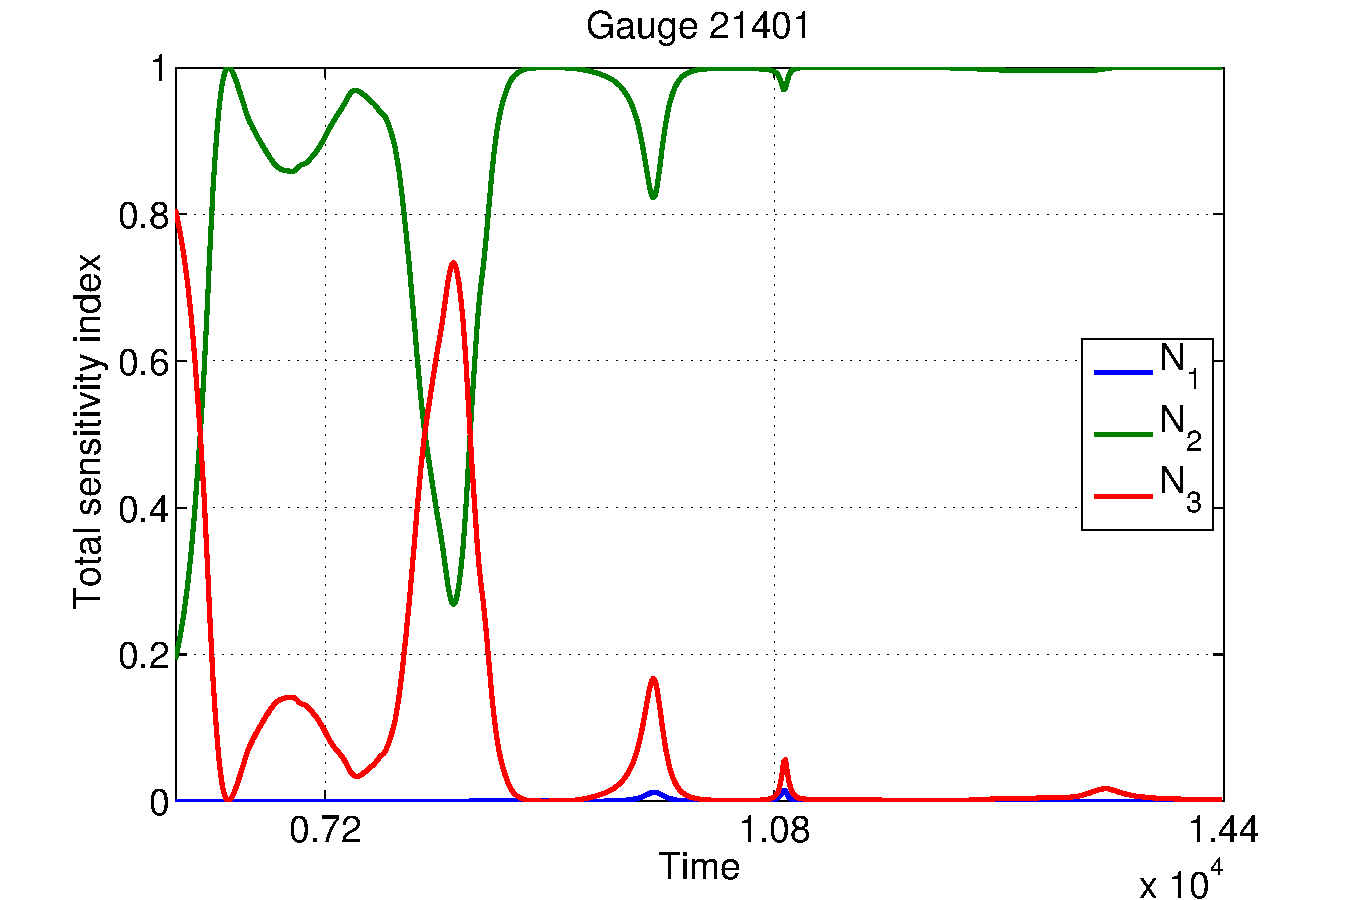
\includegraphics[width=0.475\textwidth]{./figures/sens1.pdf} &
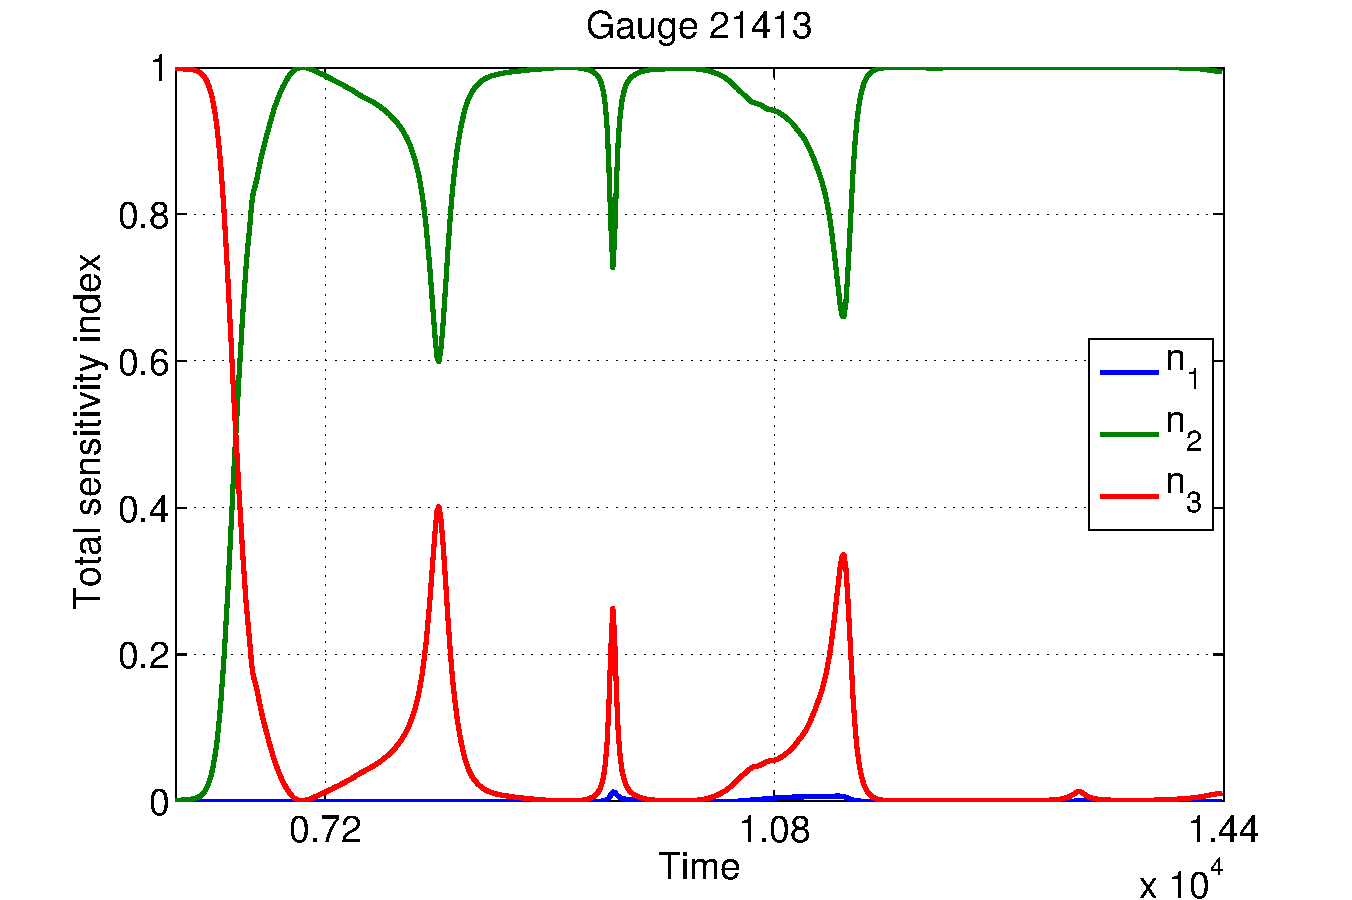
\includegraphics[width=0.475\textwidth]{./figures/sens2.pdf} \\
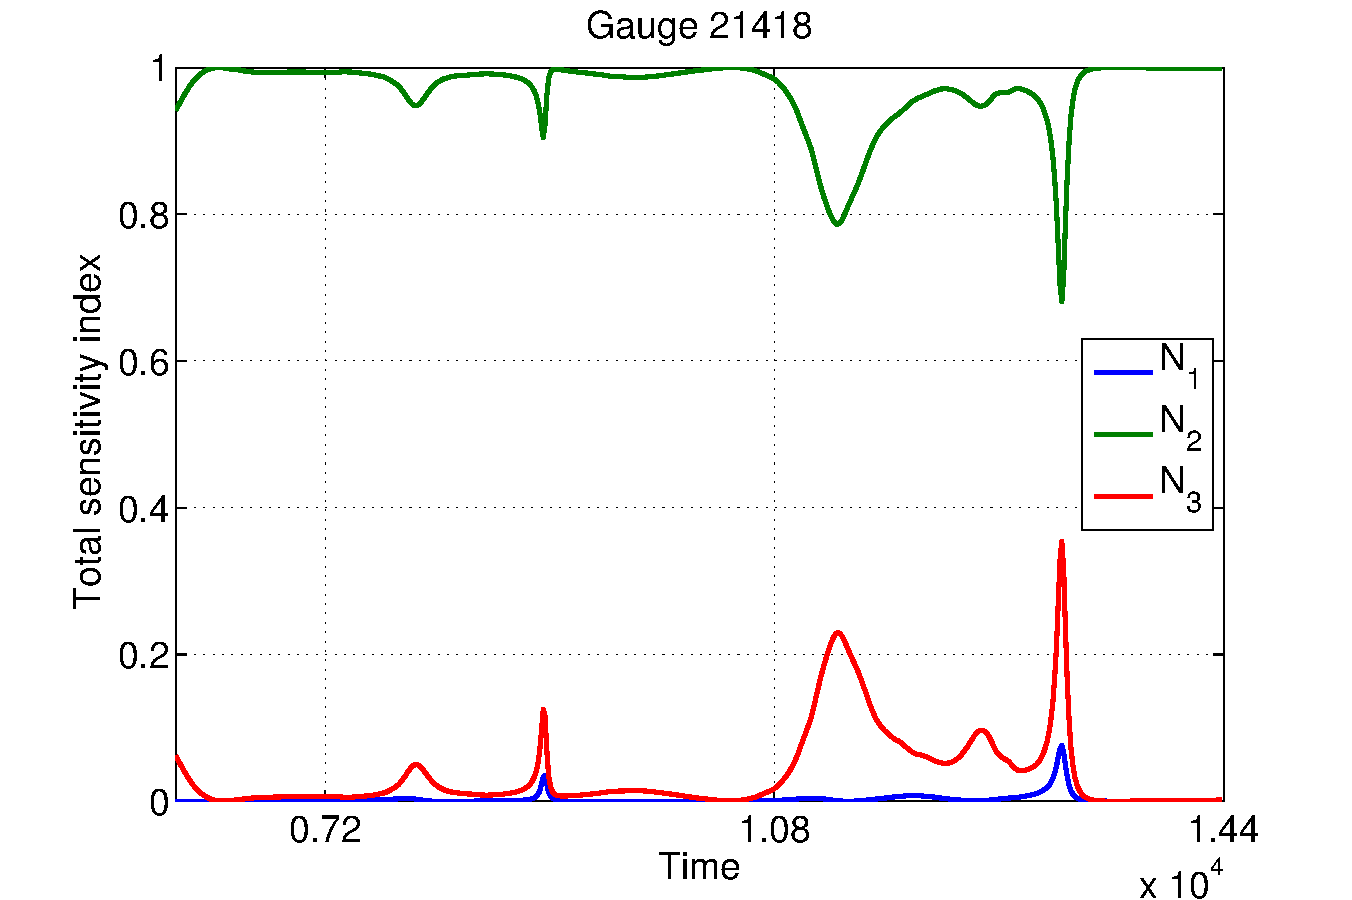
\includegraphics[width=0.475\textwidth]{./figures/sens3.pdf} &
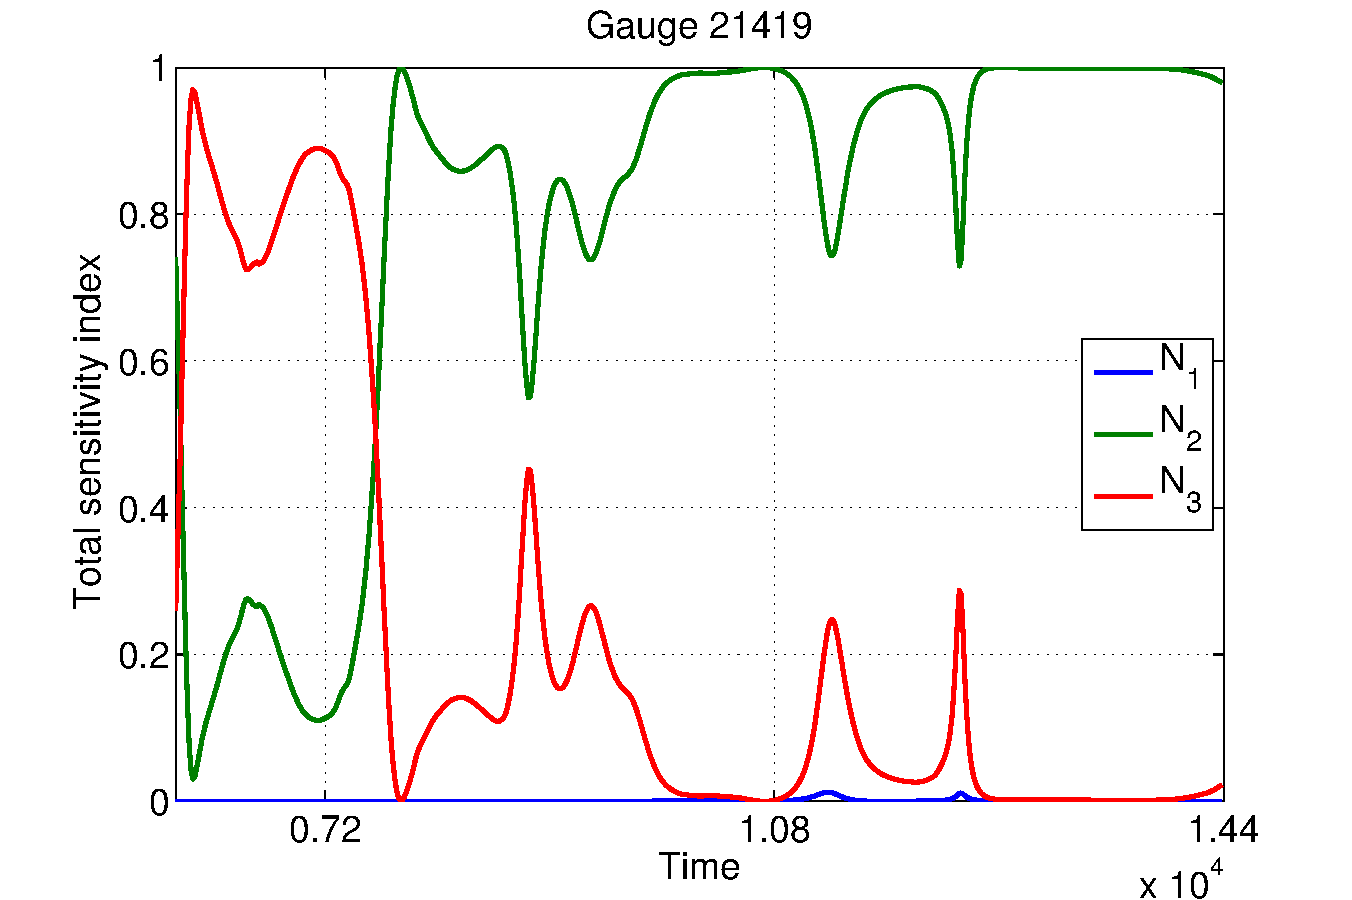
\includegraphics[width=0.475\textwidth]{./figures/sens4.pdf}
\end{tabular}
\caption{Total sensitivity index of different input parameters.}
\label{fig:sens}
\end{figure}
%%%%%%%%%%%%%%%%%%%%%%%%%%%%%%%%%%%%%%%%%%%%%%%%%%%%%%%%%%%%%%%%

\begin{figure}[ht]
\begin{tabular}{clc}
 \hspace*{-55pt}
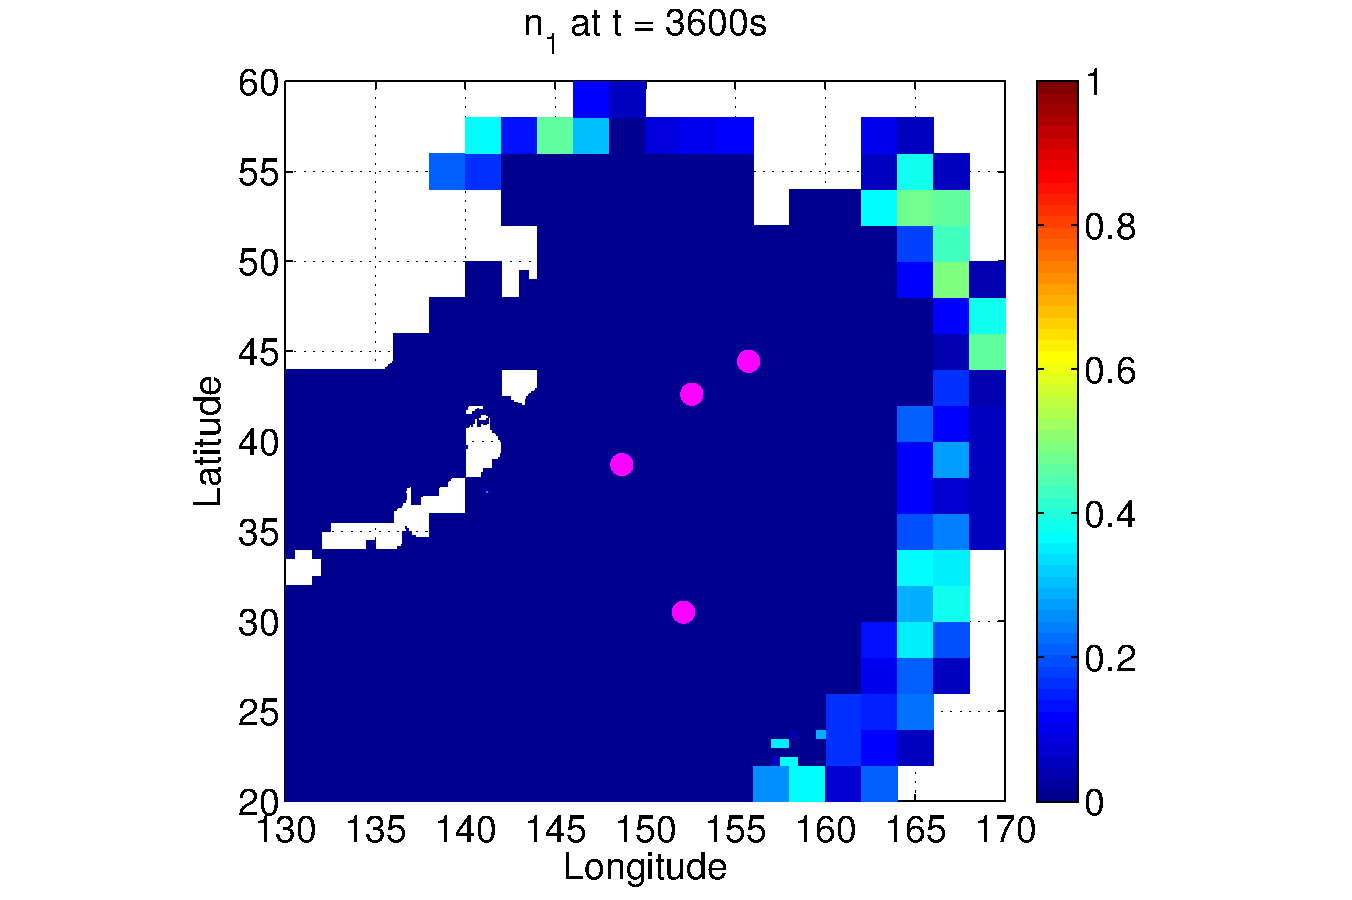
\includegraphics[width=0.45\textwidth]{./figures/T12d1.pdf} &
\hspace*{-45pt}
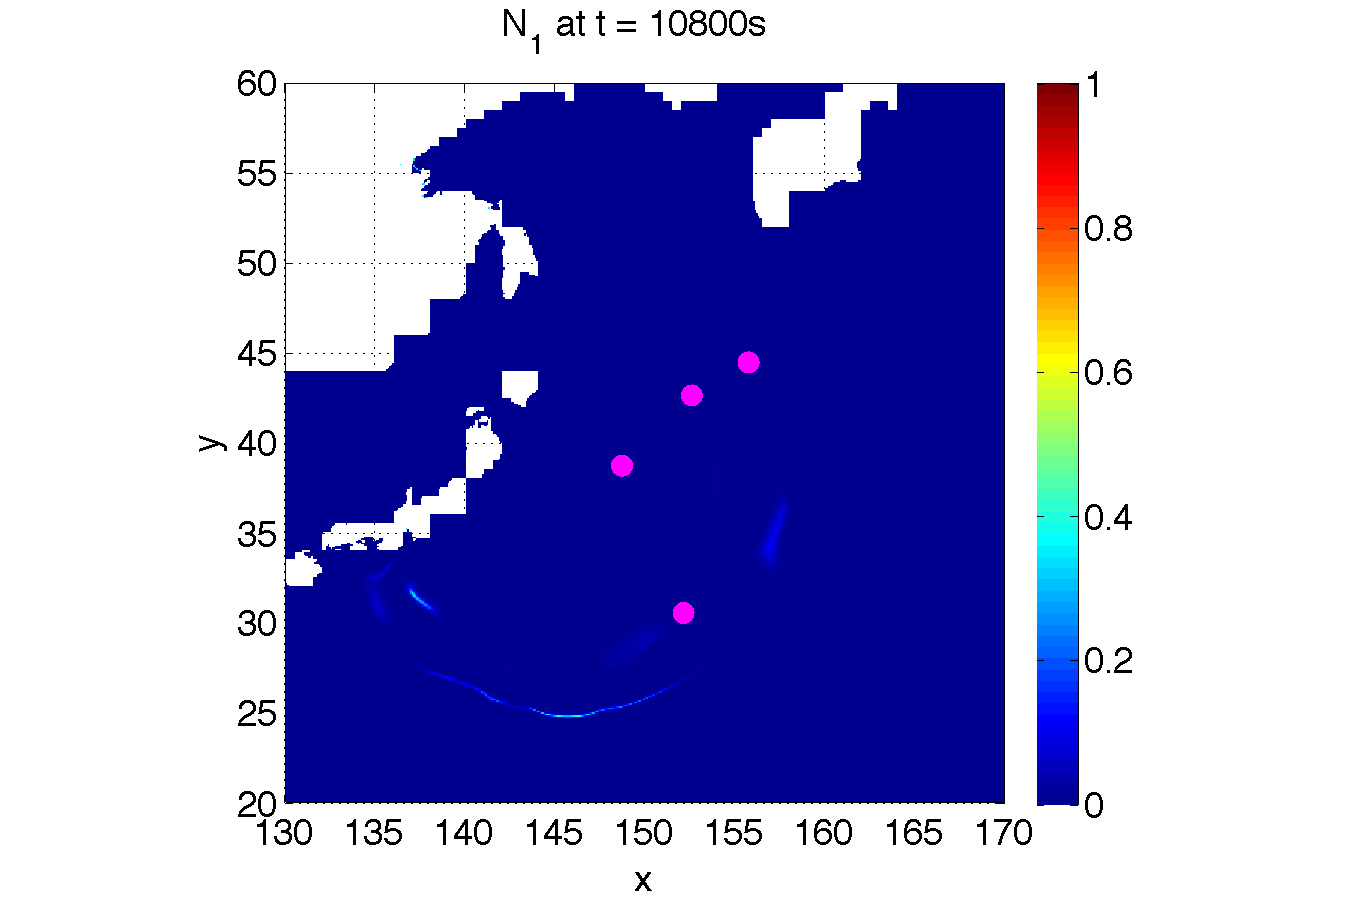
\includegraphics[width=0.45\textwidth]{./figures/T12d3.pdf} &
\hspace*{-45pt}
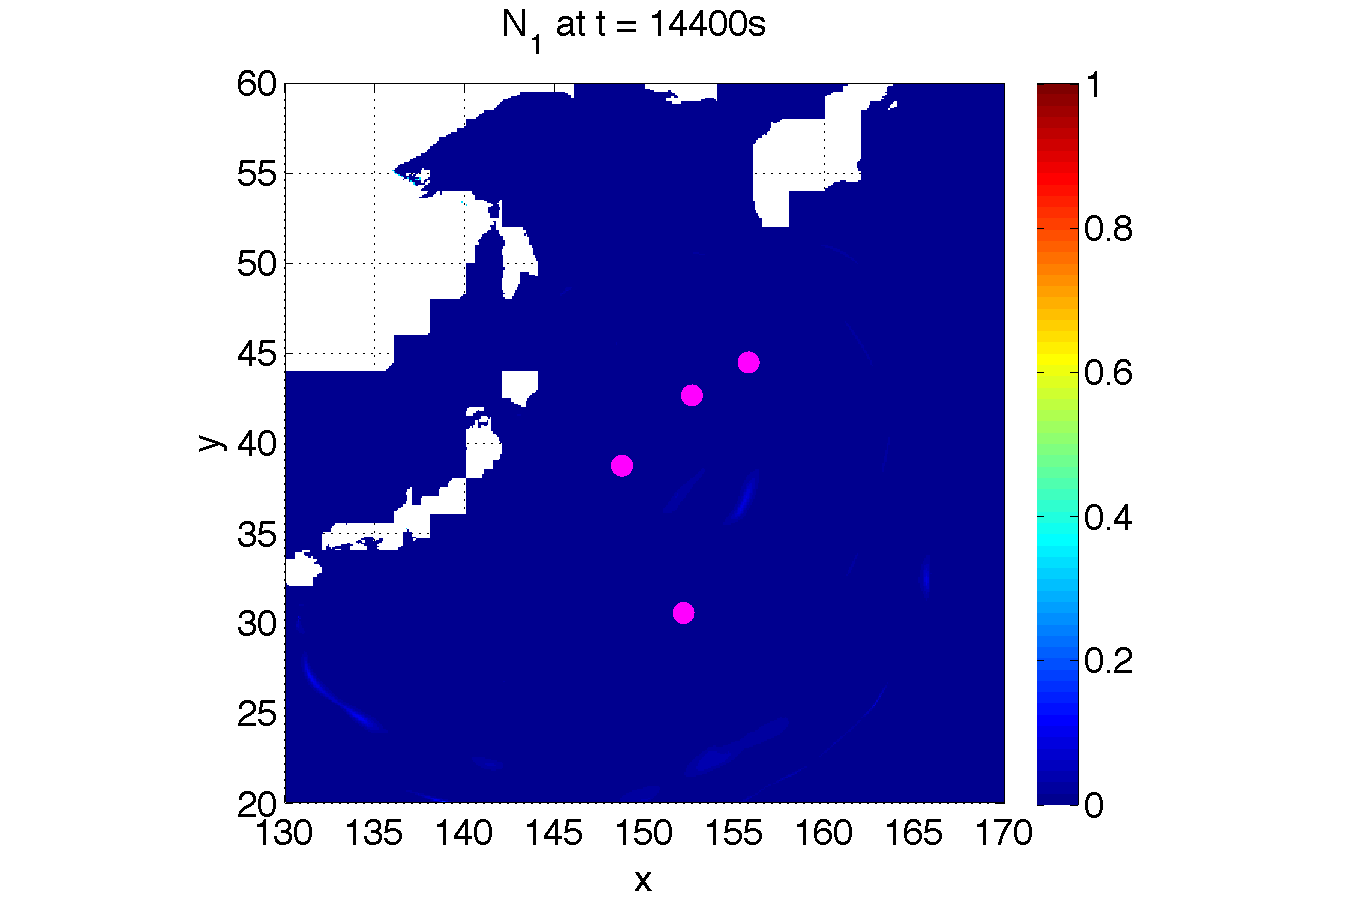
\includegraphics[width=0.45\textwidth]{./figures/T12d4.pdf} \\
\hspace*{-55pt}
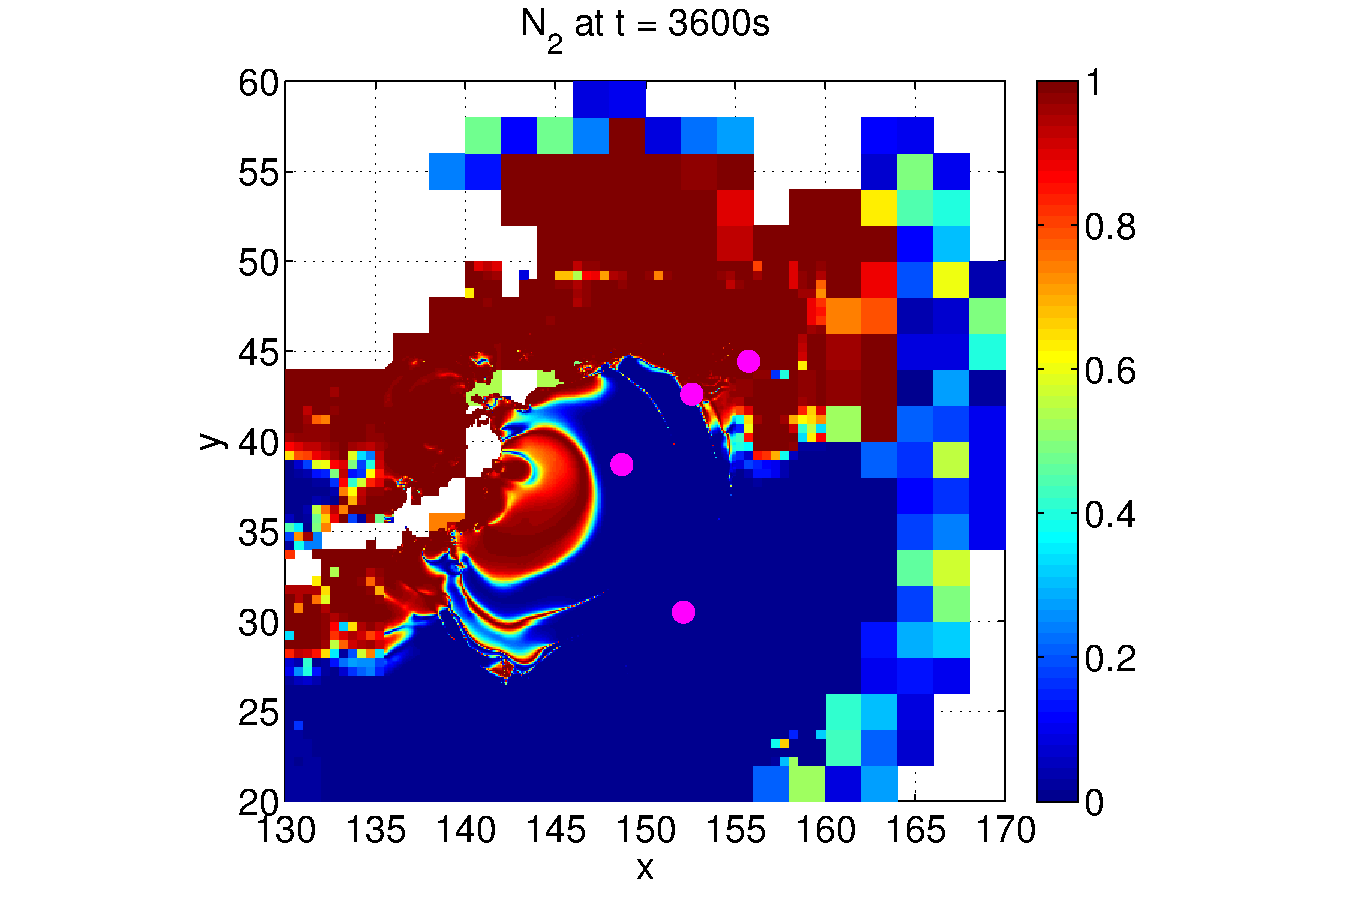
\includegraphics[width=0.45\textwidth]{./figures/T22d1.pdf} &
\hspace*{-45pt}
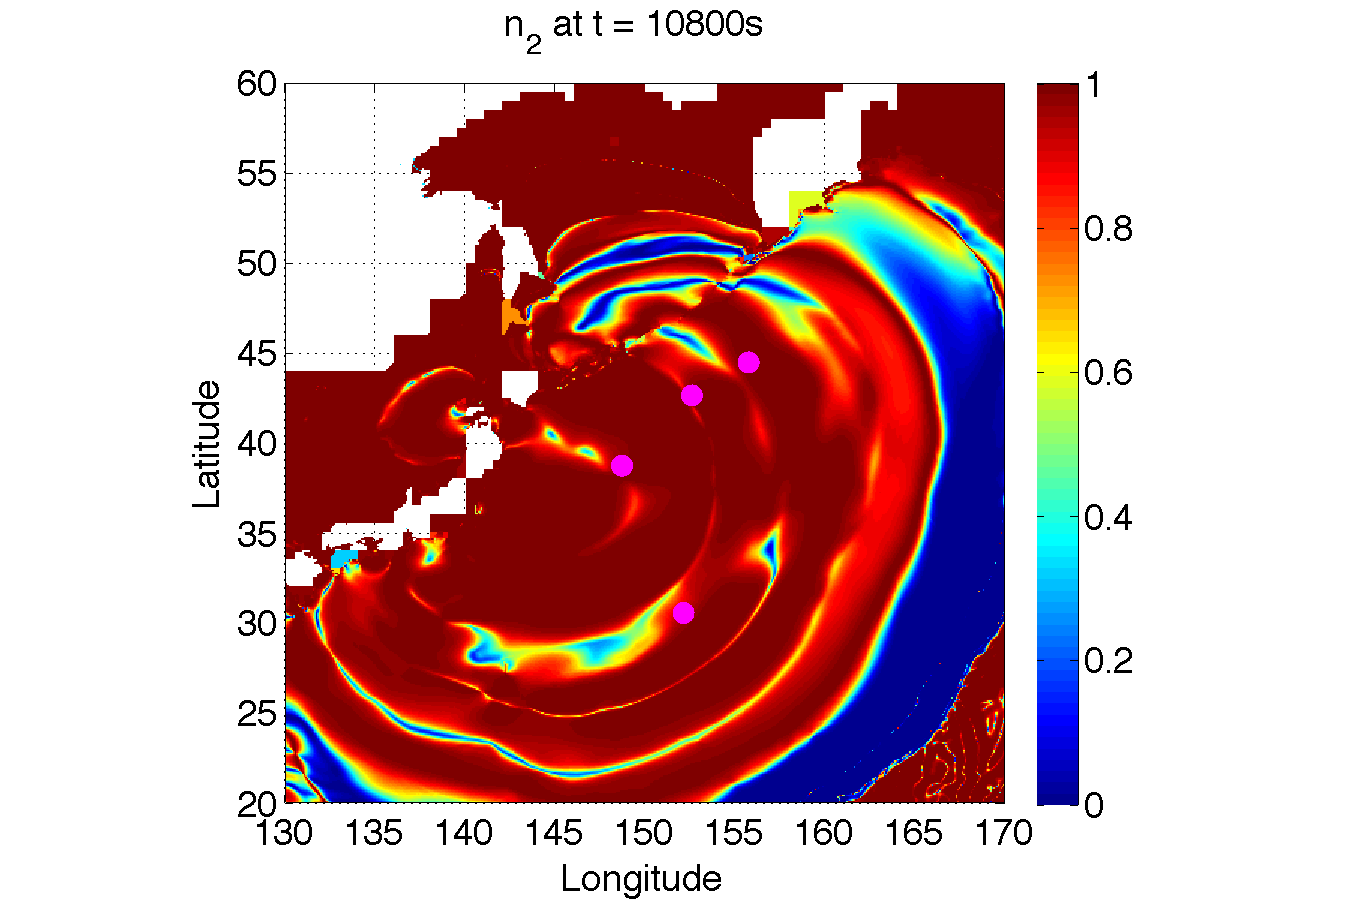
\includegraphics[width=0.45\textwidth]{./figures/T22d3.pdf} &
\hspace*{-45pt}
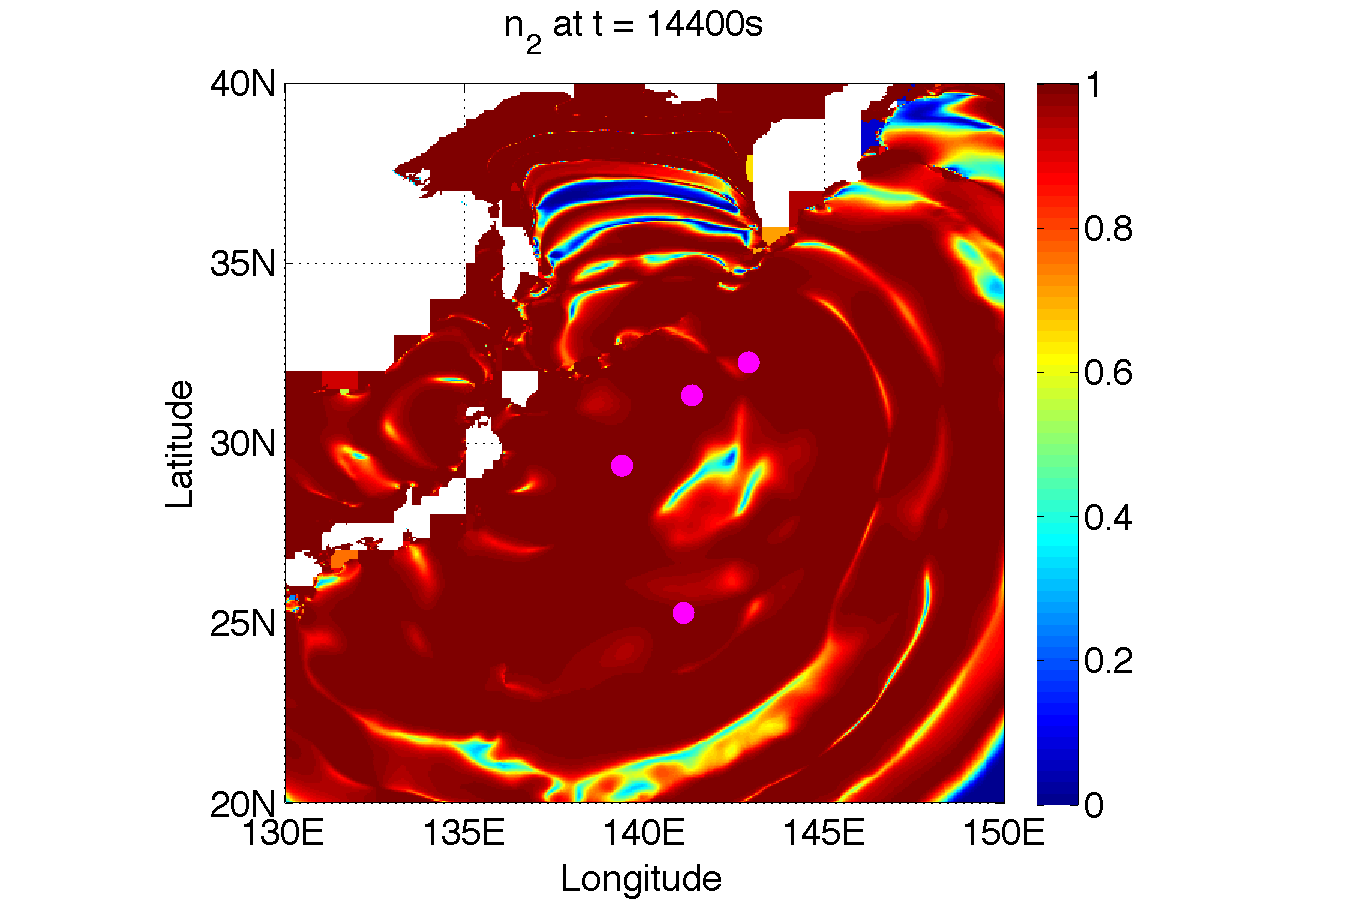
\includegraphics[width=0.45\textwidth]{./figures/T22d4.pdf} \\
\hspace*{-55pt}
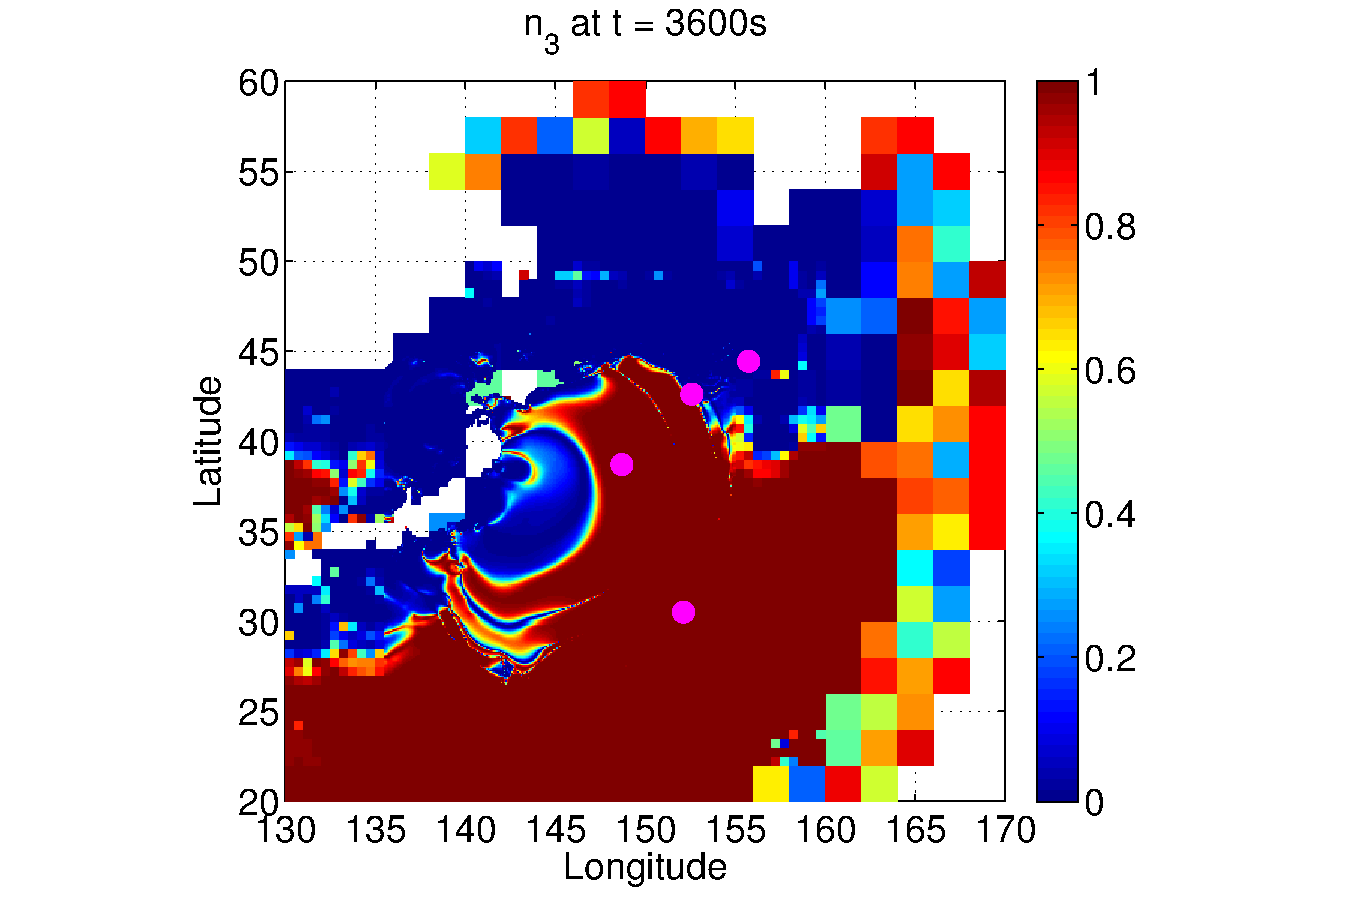
\includegraphics[width=0.45\textwidth]{./figures/T32d1.pdf} &
\hspace*{-45pt}
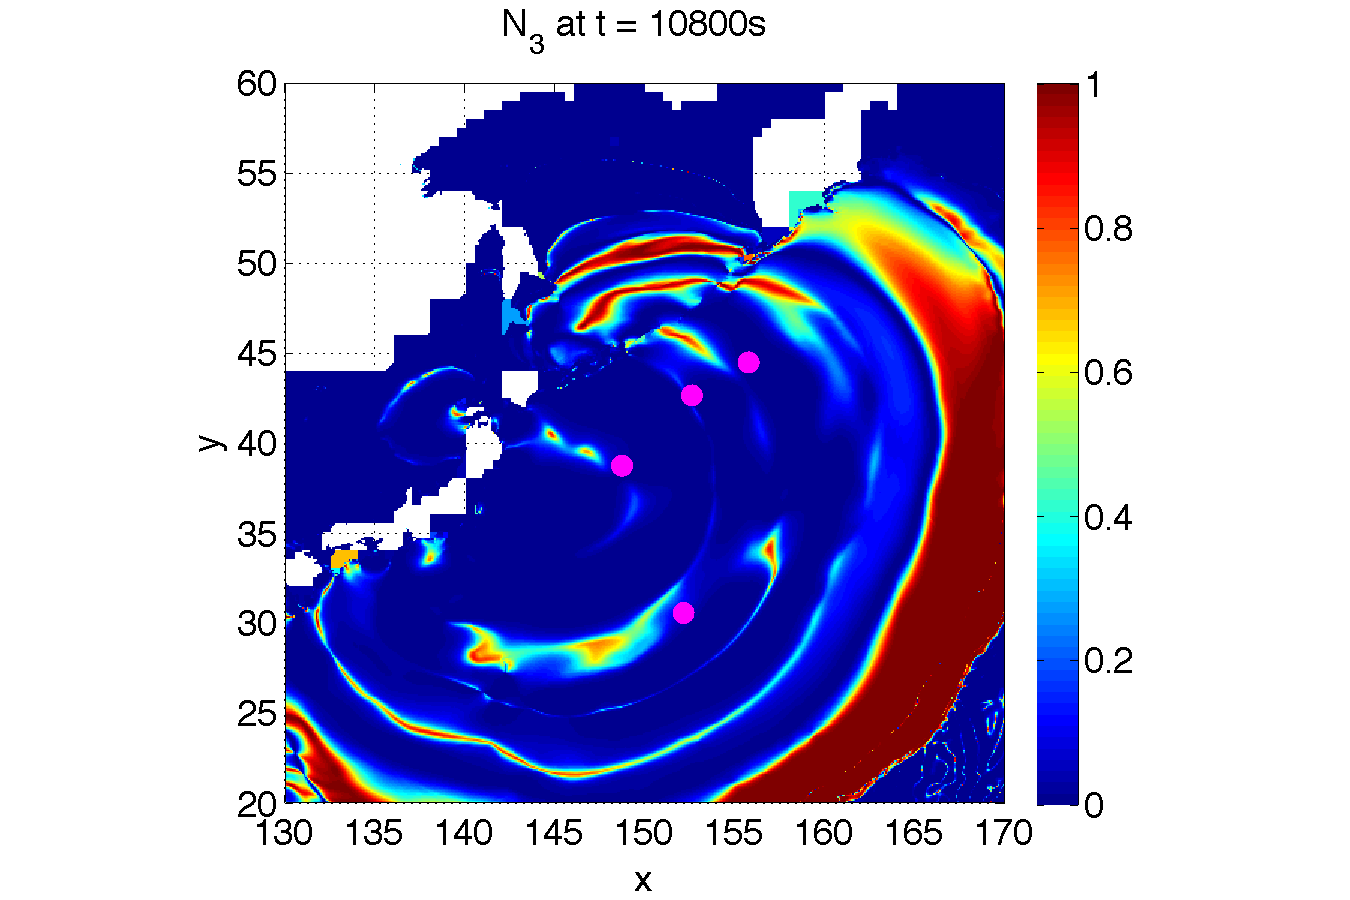
\includegraphics[width=0.45\textwidth]{./figures/T32d3.pdf} &
\hspace*{-45pt}
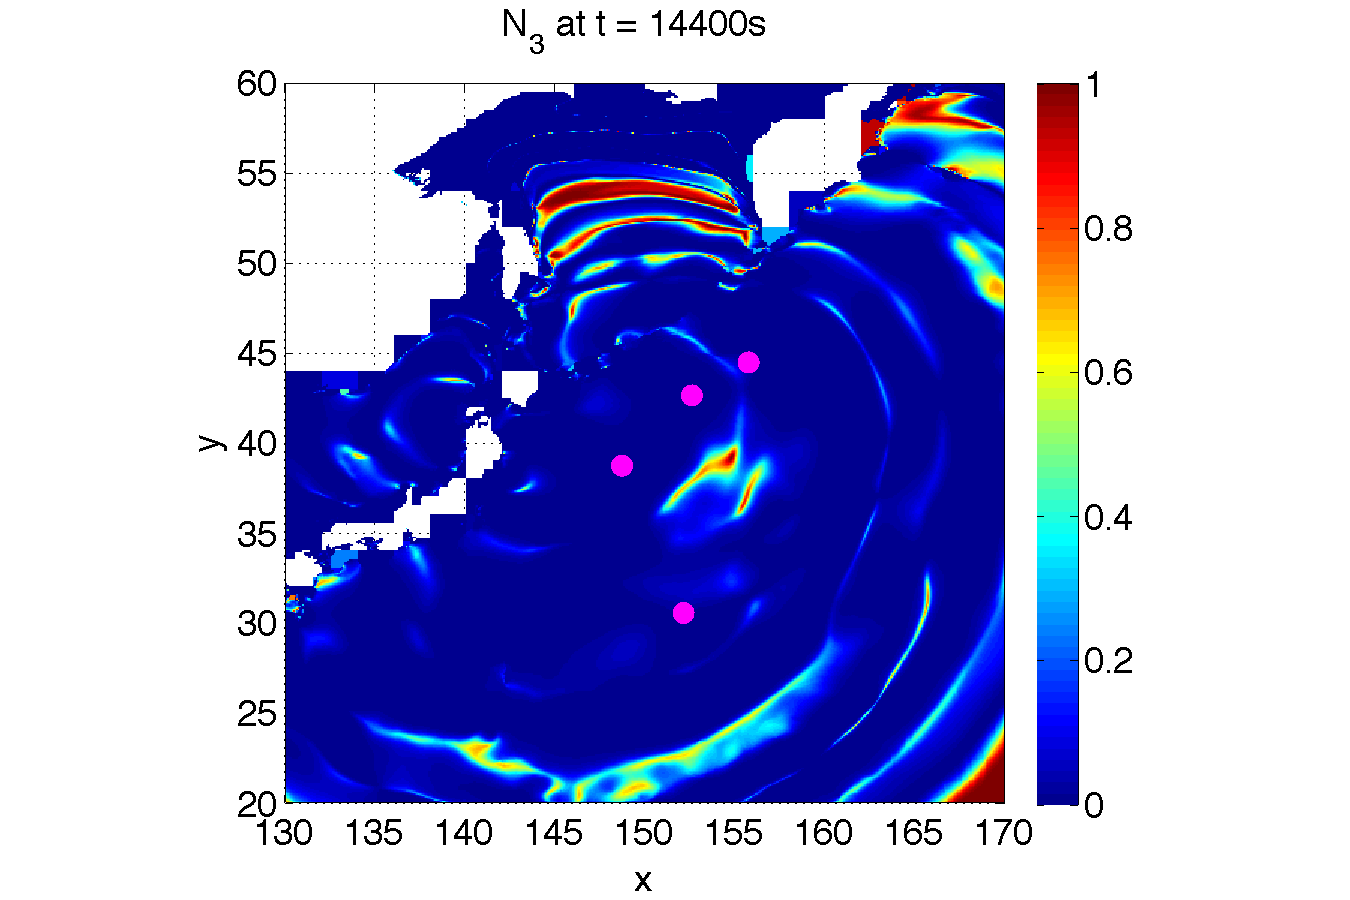
\includegraphics[width=0.45\textwidth]{./figures/T32d4.pdf}
\end{tabular}
\caption{Total sensitivity index for $n_1$ (top row) $n_2$ (center row) and $n_3$ (bottom row)
 at different times as indicated.}
\label{fig:sens2d}
\end{figure}
%%%%%%%%%%%%%%%%%%%%%%%%%%%%%%%%%%%%%%%%%%%%%%%%%%%%%%%%%%%%%%%%
\begin{figure}[ht]
\centering

\begin{tabular}{clcl}
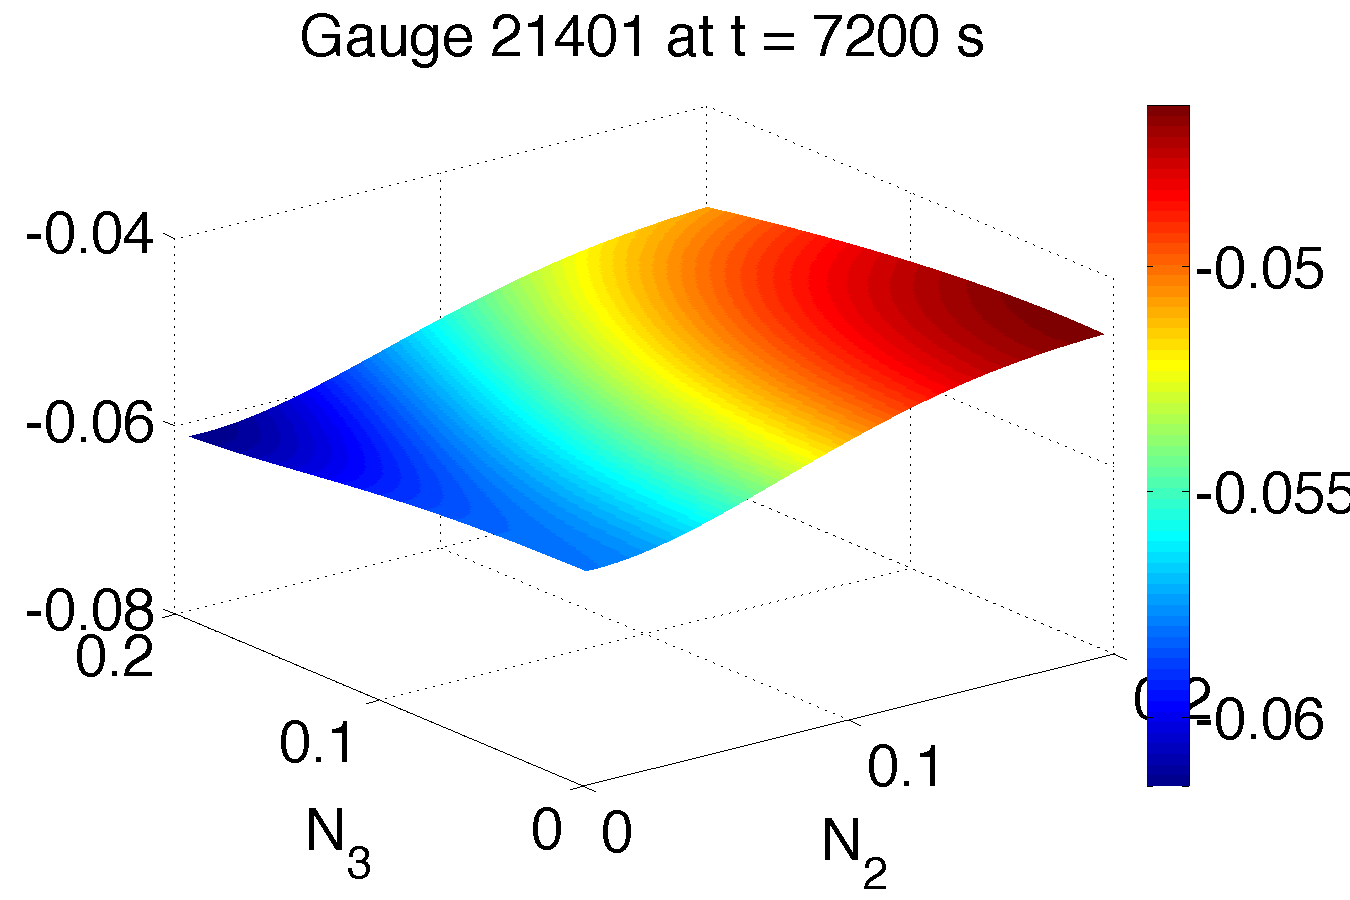
\includegraphics[width=0.5\textwidth]{./figures/response_i1_t2.pdf} &
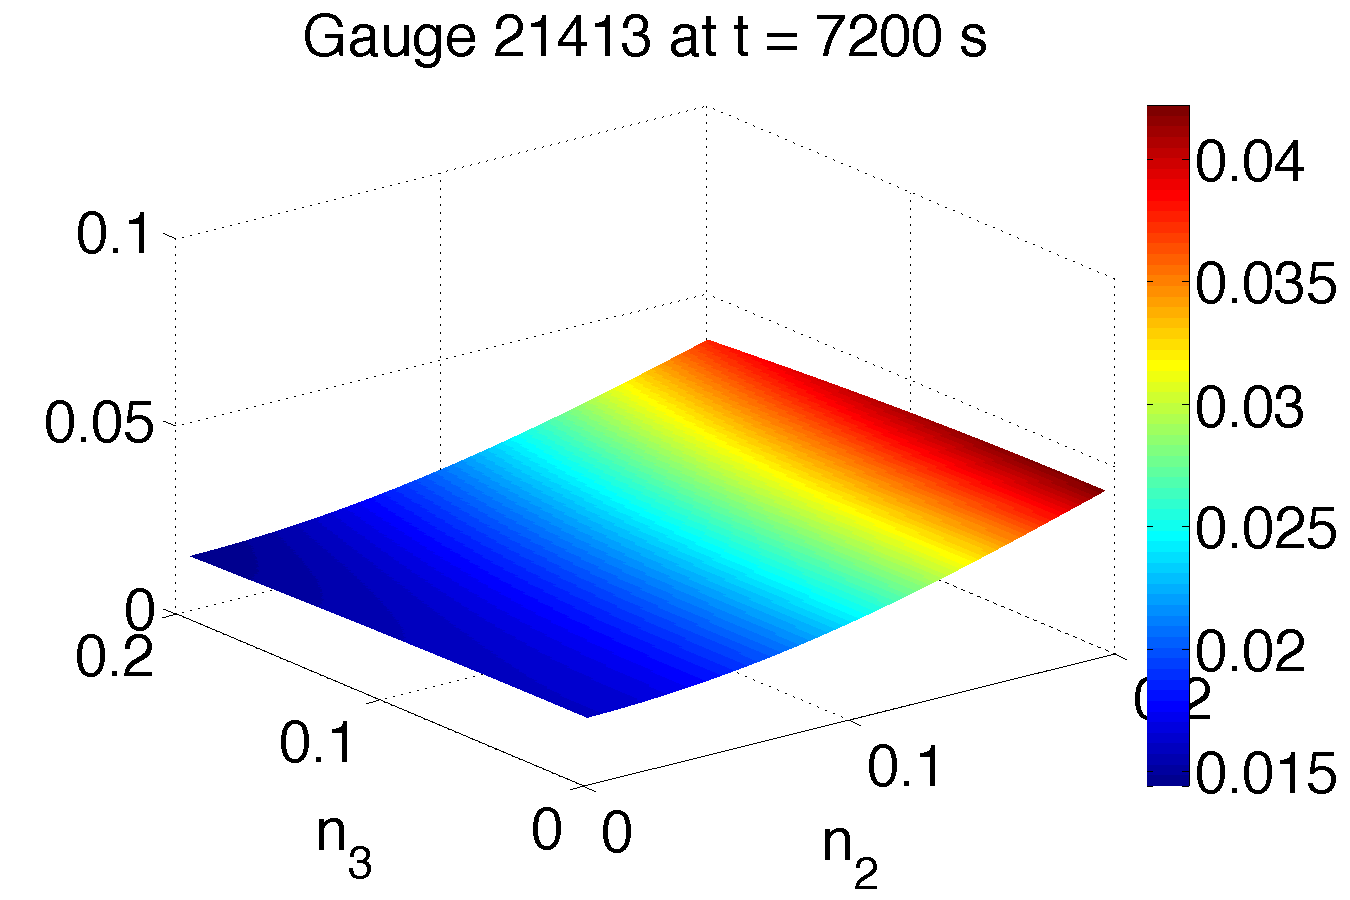
\includegraphics[width=0.5\textwidth]{./figures/response_i2_t2.pdf} \\
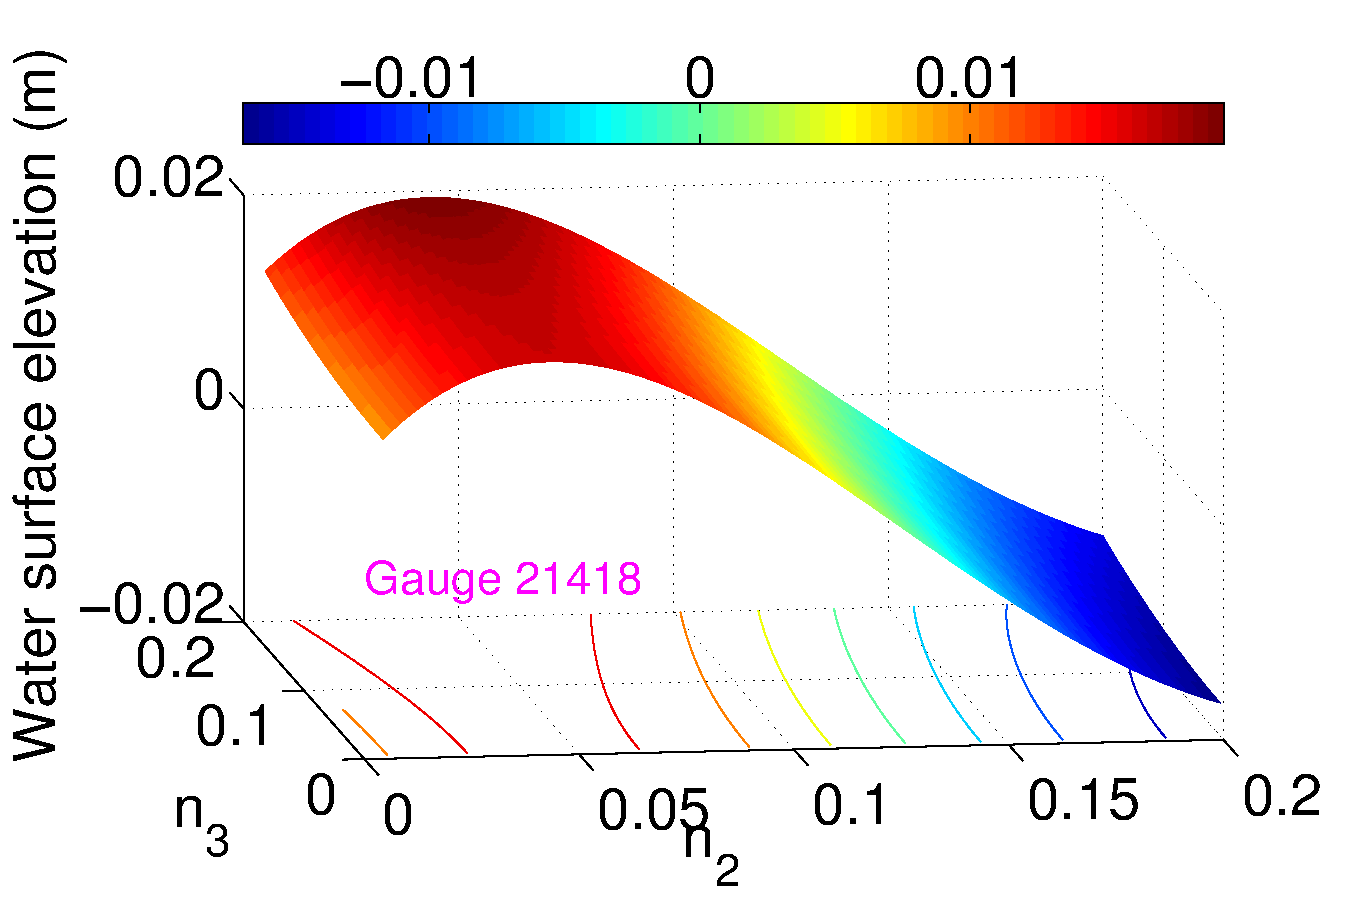
\includegraphics[width=0.5\textwidth]{./figures/response_i3_t2.pdf} &
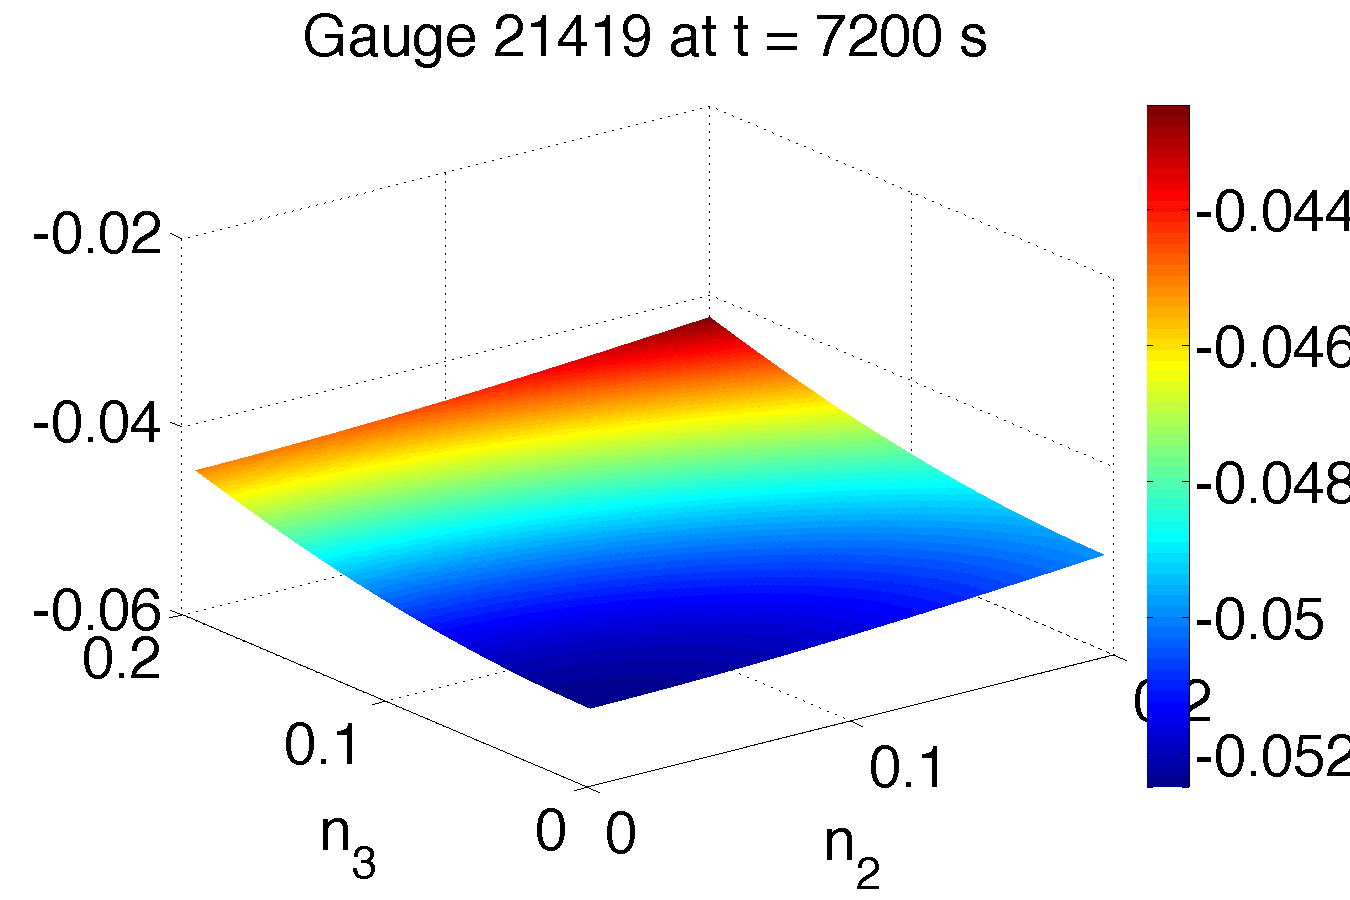
\includegraphics[width=0.5\textwidth]{./figures/response_i4_t2.pdf}
\end{tabular}
\caption{Response surface of water surface elevation at the different gauge locations at t = 7200 s
as function of $n_2$ and $n_3$, with fixed $n_1=0.035$}.
\label{fig:response2}
\end{figure}
%%%%%%%%%%%%%%%%%%%%%%%%%%%%%%%%%%%%%%%%%%%%%%%%%%%%%%%%%%%%%%%%
%\begin{figure}[ht]
%\centering
%
%\begin{tabular}{clcl}
%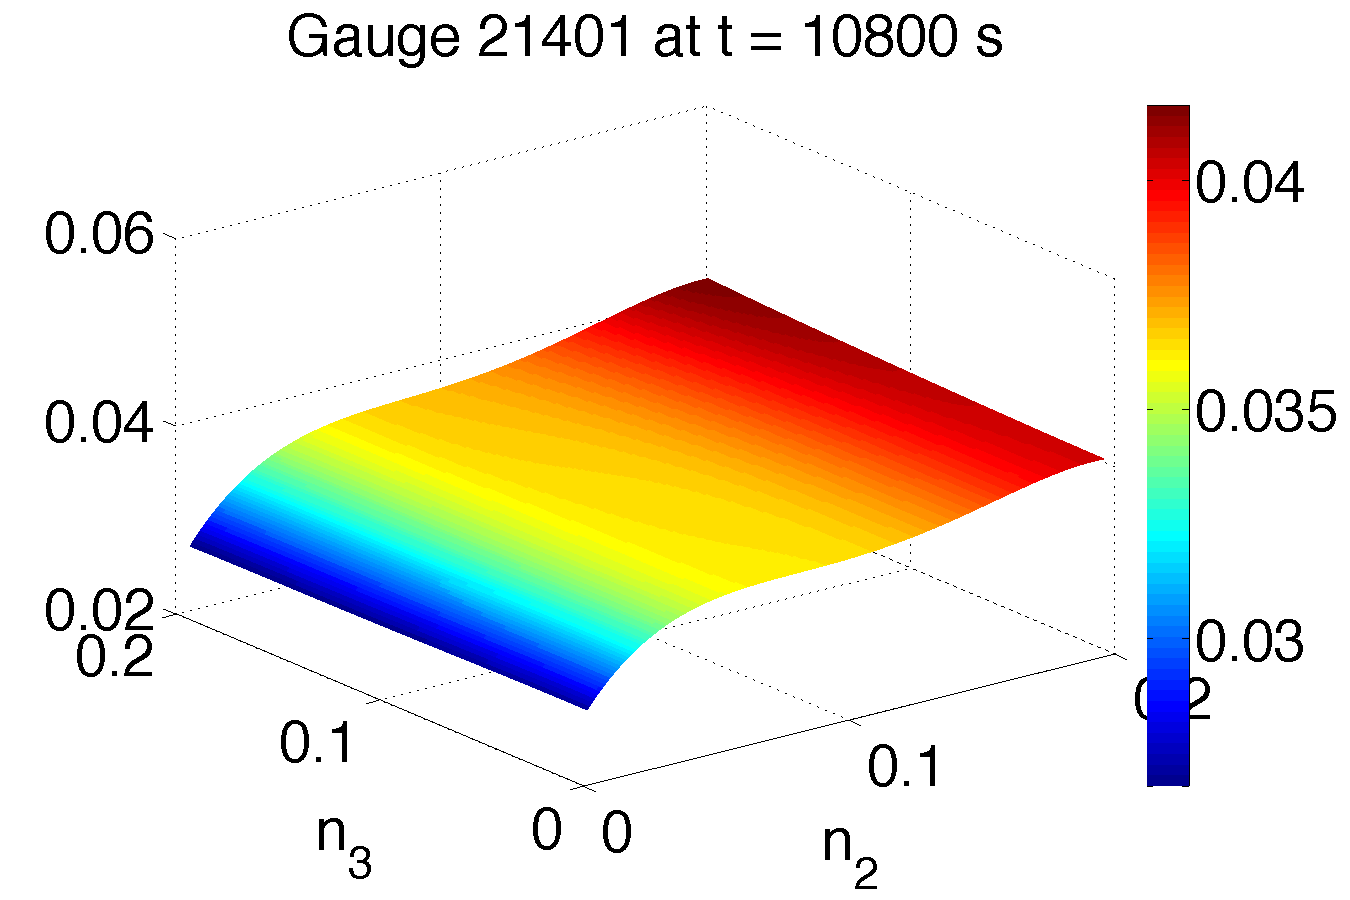
\includegraphics[width=0.5\textwidth]{./figures/response_i1_t3.pdf} &
%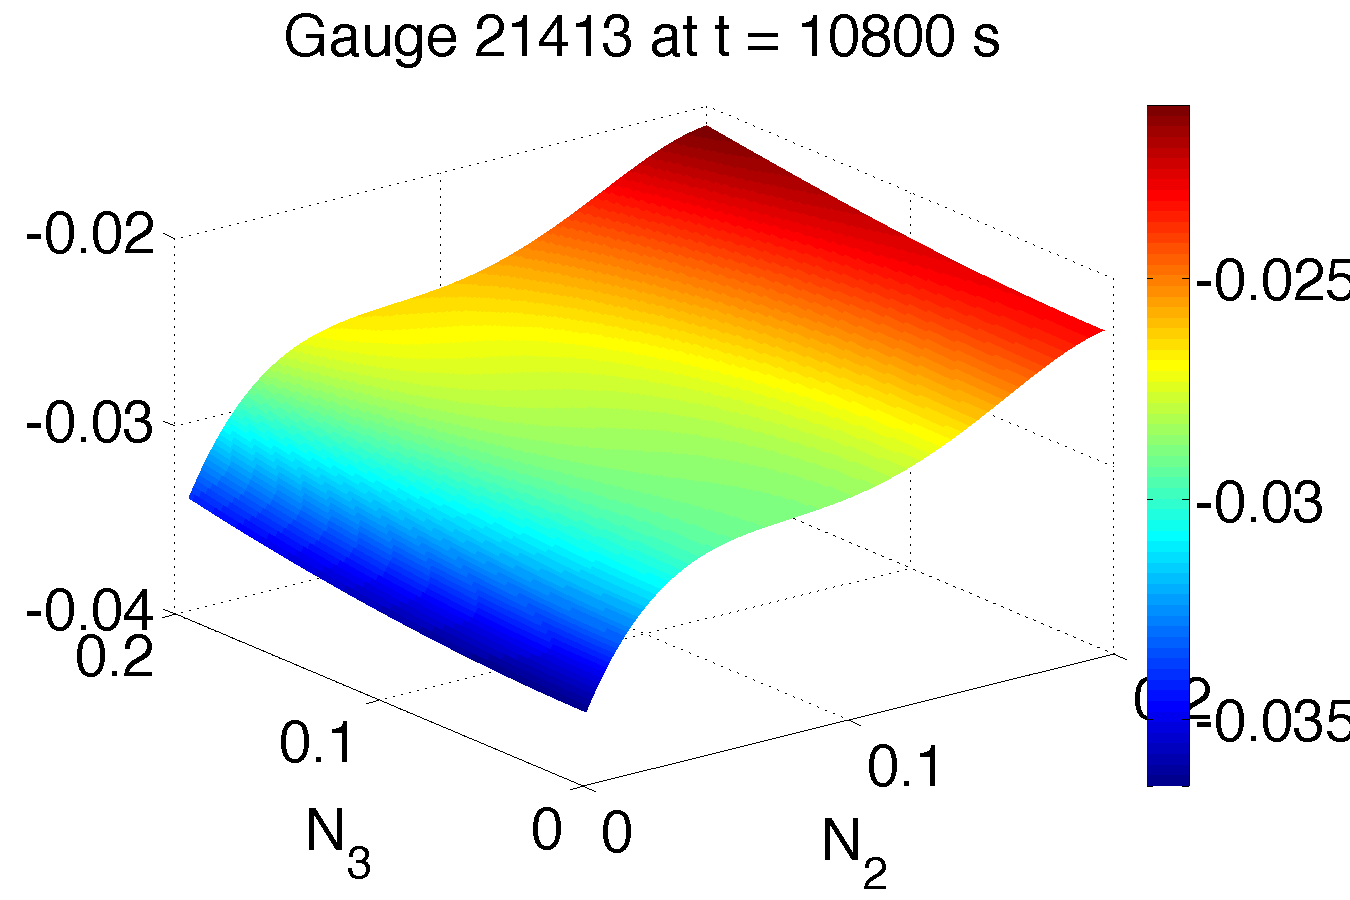
\includegraphics[width=0.5\textwidth]{./figures/response_i2_t3.pdf} \\
%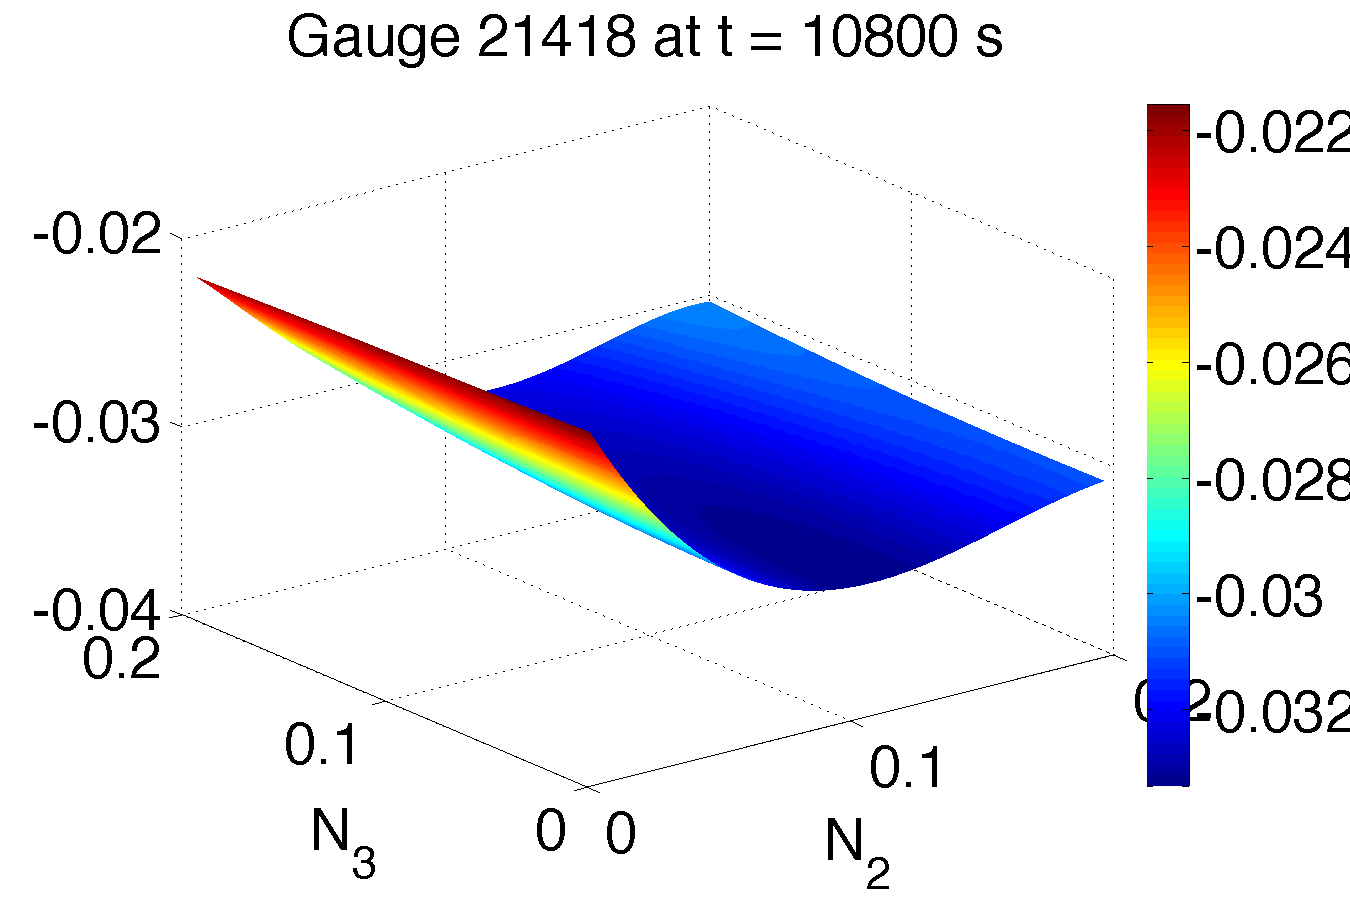
\includegraphics[width=0.5\textwidth]{./figures/response_i3_t3.pdf} &
%\includegraphics[width=0.5\textwidth]{./figures/response_i4_t3.pdf}
%\end{tabular}
%\caption{Response surface of water surface elevation at the different gauge locations at t = 14400 s.}
%\label{fig:response3}
%\end{figure}
%%%%%%%%%%%%%%%%%%%%%%%%%%%%%%%%%%%%%%%%%%%%%%%%%%%%%%%%%%%%%%%%
\begin{figure}[ht]
\centering
\includegraphics[width=0.575\textwidth]{./figures/scatter.pdf} 
\caption{Scatter plot of measured water surface elevation against their \geoclaw
model counterparts during Tsunami \tohoku. The data points are colored 
differently for the different gauges as indicated in the legend. }
\label{fig:scatter}

\end{figure}  
%%%%%%%%%%%%%%%%%%%%%%%%%%%%%%%%%%%%%%%%%%%%%%%%%%%%%%%%%%%%%%%%
\begin{figure}[ht]
\begin{tabular}{clc}
\includegraphics[width=0.475\textwidth]{./figures/chain_p1.pdf} &
\includegraphics[width=0.475\textwidth]{./figures/chain_p2.pdf} \\
\includegraphics[width=0.475\textwidth]{./figures/chain_p3.pdf} &
\includegraphics[width=0.475\textwidth]{./figures/chain_s1.pdf}
\end{tabular}
\caption{Chain samples for the three Manning's $n$ coefficients $n_1,n_2,n_3$ and $\sigma^2$
the variance between simulations and observations. The vertical lines corresponds to the
burn-in iterations.}
\label{fig:mcmc} 
\end{figure}
%%%%%%%%%%%%%%%%%%%%%%%%%%%%%%%%%%%%%%%%%%%%%%%%%%%%%%%%%%%%%%%%
 \begin{figure}[ht]
        \begin{tabular}{clc}
\includegraphics[width=0.475\textwidth]{./figures/pdf_p1.pdf} &
\includegraphics[width=0.475\textwidth]{./figures/pdf_p2.pdf} \\
\includegraphics[width=0.475\textwidth]{./figures/pdf_p3.pdf} &
\includegraphics[width=0.475\textwidth]{./figures/pdf_s1.pdf}
        \end{tabular}
        \caption{Posterior distributions for the three Manning's $n$ coefficients $n_1,n_2,n_3$ 
and $\sigma^2$ the variance between simulations and observations.}
\label{fig:pdfs} 
        \end{figure}
